\documentclass[pdflatex,sn-mathphys,Numbered]{sn-jnl}

\usepackage{graphicx}
\graphicspath{{figures/}{figures/}}
\makeatletter
\def\input@path{{tables/}{tables/}}
\makeatother
\usepackage{booktabs}
\usepackage{amsmath,amssymb,amsfonts}
\usepackage{amsthm}
\usepackage[title]{appendix}
\usepackage{longtable}
\usepackage{adjustbox}
\usepackage{array}
\usepackage{algorithmicx}
\usepackage{algpseudocode}
\usepackage{listings}

% Symbols for table checks
\newcommand{\cmark}{\checkmark}
\newcommand{\xmark}{--}

\newtheorem{proposition}{Proposition}

\hypersetup{colorlinks=true, linkcolor=blue, citecolor=blue, urlcolor=blue, 
pdftitle={Characterizing Micro-Architectural Memory Pressure Stall Dynamics, Dynamic Cgroup V2 Overcommit, and Tail-Resilient Eviction Avoidance in Dense Cloud Multi-Tenancy}, 
pdfauthor={Devarsh Patel, Adarsh Singh, Umamaheshwari M}, 
pdfkeywords={Cloud Computing, Memory Overcommit, Cgroups v2, Pressure Stall Information, Tail Latency, Extreme Value Theory, Direct Reclamation, MGLRU}}

\begin{document}

\title[Memory Pressure Stall Dynamics in Cloud Multi-Tenancy]{Characterizing Micro-Architectural Memory Pressure Stall Dynamics, Dynamic Cgroup V2 Overcommit, and Tail-Resilient Eviction Avoidance in Dense Cloud Multi-Tenancy}

\author[1]{\fnm{Devarsh} \sur{Patel}}\email{devarsh.patel2024@vitstudent.ac.in}
\author[1]{\fnm{Adarsh} \sur{Singh}}\email{adarsh.singh2024b@vitstudent.ac.in}
\author*[1]{\fnm{Umamaheshwari} \sur{M}}\email{umamaheshwari.m@vit.ac.in}

\affil[1]{\orgdiv{School of Computer Science and Engineering (SCOPE)}, \orgname{Vellore Institute of Technology (VIT)}, \orgaddress{\city{Vellore}, \state{Tamil Nadu}, \country{India}}}

\abstract{
In modern cloud multi-tenant infrastructure, DRAM accounts for 40\%--50\% of server capital expenditure (CapEx), in real-world scenarios; cloud orchestrators routinely maximize physical memory density by overcommitting memory, through Linux cgroup v2 control boundaries, to the significant degree, on the whole; truly, yet, standard static overcommit configurations trigger severe, non-linear tail-latency cascades when concurrent tenants experience sudden bursts in their working sets; and thus, simultaneously, physical host CPU utilization is remaining under 40\%, at least for now. Under all these conditions, under the conditions, we introduce any second empirical and theoretical study of kernel direct memory reclamation dynamics, across the high-density multi-tenant cloud workloads in this examination, at least in belief, in actual application. Under all this conditions, under the conditions, applying high-frequency (sub-10 millisecond) event-driven monitoring of Linux Kernel Pressure Stall Information (PSI), we uncover that pre-OOM direct reclamation stalls in kernel \texttt{shrink\_node()} amplify P99.9 memory allocation latency by more than three orders of extent (from $23.8\ \mu\text{s}$ to $48,400\ \mu\text{s}$ / $48.4\text{ ms}$), broadly speaking. Viewed through this lens, anonymous heap expansion against file-backed page-cache thrashing under the modern Linux 6.8 Multi-Gen LRU (MGLRU) versus classic Dual-LRU subsystems is assessed, and formalize parametric tail distributions applying Extreme Value Theory (EVT) Generalized Pareto Distributions (GPD) and analytically derive the closed-form Safe Overcommit Capacity Frontier $\Omega^*(\alpha, L_{\text{SLA}}, \beta_{\text{burst}})$, at least in practice. In this broader context, along the dimensions, building on this gather, under all the conditions, judged on any company bare-metal cloud server ($M_{\text{DRAM}} = 192\text{ GB}$ container domain), direct reclamation tail stalls by $410.2\times$ are greatly hidden by PSI-Shed, reaching this P99.9 latency of $118.0\ \mu\text{s}$ (Cohen's $d = 1.48$, Tail Cliff's $\delta_{\text{tail}} = 0.987$) and safely expanding the overcommit frontier from $\Omega = 1.15$ to $\Omega = 1.68$ while keeping $99.7\%$ of opportunistic batch analytics throughput, on the whole. Within this framework, finally, we design, execute and gauge \textbf{PSI-Shed}, one acceleration-aware user-space memory controller that dynamically is relieving \texttt{memory.high} boundaries grounded in discrete-time PSI acceleration $\mathbf{a}_{\text{some}}(t) = d^2(\text{PSI})/dt^2$ and reclamation scan efficiency $\mathcal{E}_{\text{reclaim}}$, to this significant degree, at least in practice.
}

\keywords{Cloud Computing, Memory Overcommit, Linux Cgroups v2, Pressure Stall Information (PSI), Tail Latency, Extreme Value Theory, Multi-Gen LRU, Proactive Mitigation}

\maketitle

\section{Introduction}
\label{sec:intro}

\subsection{The Economic Imperative of DRAM Overcommit in Cloud Computing}
That is, modern hyperscale and business private cloud datacenters operate, under intense economic pressures regulated by server hardware procurement costs \cite{barham2003xen, waldspurger2002esx}, on the whole, and across warehouse-scale compute nodes, dynamic random-access memory (DRAM) constitutes between 40\% and 50\% of total server capital expenditure (CapEx) and consumes roughly 25\%--30\% of whole-node operational power \cite{verma2015borg, tirmazi2020borg}, in many respects. Because, typical production containers provision memory for worst-case seasonal peak utilization, average physical DRAM utilization, across cloud clusters routinely hovers between 35\% and 55\% \cite{cortez2017resourcecentral, rzadca2020autopilot}, broadly speaking. In this broader context, hyperscale operators have been driven by this widespread allocation slack to embrace memory overcommit architectures, wherein the aggregate memory limits named to co-located tenants greatly exceed physical DRAM capacity ($\Omega = \sum M_{\max}^{(i)} / M_{\text{DRAM}} > 1.0$) \cite{lagarcavilla2019far, li2023pond}, at least for now.

To manage overcommitted multi-tenant density, modern container engines (e.g., Kubernetes, containerd) rely on the unified Linux control group hierarchy (cgroup v2) \cite{weiner2022tmo}, at least for now. In this broader context, along all all these dimensions, from this viewpoint, taken together, building on this finding, under the quiescent operation, cold clean page-cache pages and inactive anonymous folios are continuously reclaimed by asynchronous kernel background daemons (\texttt{kswapd}), upholding allocatable headroom above physical zone high watermarks without changing running tasks \cite{liu2021hpc}, to one more significant degree, at least in practice. Cgroups v2 supplies memory watermarks (\texttt{memory.min}, \texttt{memory.low}, \texttt{memory.high}, and \texttt{memory.max}) intended to partition DRAM among latency-critical interactive microservices, streaming file-cache buffers, and opportunistic batch workloads \cite{amaro2020far, ruan2020aifm}, in actual application.

\subsection{The Pre-OOM Direct Reclamation Cliff vs. The Binary OOM Fallacy}
Without question, one widespread fallacy in cloud operations is that memory overcommit failures are only binary events dictated by the Linux Out-Of-Memory (OOM) killer (\texttt{oom-killer}) \cite{chen2019parties, gu2017infiniswap}, at least in law; also, thus, system administrators often suppose that so long as one application remains below its hard limit (\texttt{memory.max}), memory allocations routinely proceed at near-zero latency, in this principal, at least for now. 

To be precise, our empirical telemetry is broadly sharing that this suppose crashes catastrophically in multi-tenant environments; more correctly, when concurrent tenants burst their memory footprint beyond the host zone watermark (\texttt{WMARK\_LOW}), the asynchronous background thread \texttt{kswapd} is overwhelmed, at least empirically. In parallel with this, building on this see, taken together, within this framework, any user thread trying to allocate anonymous heap memory or tackle one more soft page fault is trapped synchronously inside the kernel memory allocator via \texttt{do\_try\_to\_free\_pages()} and \texttt{shrink\_node()} \cite{weiner2022tmo} at this moment; this effect, which we name the \textit{Pre-OOM Direct Reclamation Cliff}---forces interactive user-space threads to blockingly scan, lock acquisitions, and dirty page writebacks, at least empirically. So memory allocation latency explodes from token microsecond durations ($15$--$35\ \mu\text{s}$) to tens of milliseconds ($40$--$250\text{ ms}$), at least in practice, and in the interim, aggregate host CPU utilization is remaining under 40\% \cite{dean2013tailatscale}, at least empirically; all things considered. In parallel with this, viewed through this lens, also thus, for latency-critical services bound by strict tail service level agreements (SLAs), this direct reclamation stalling findings in severe service degradation, timeouts and cascading microservice failures long before the kernel OOM killer fires, in many respects.

\begin{figure*}[t]
\centering
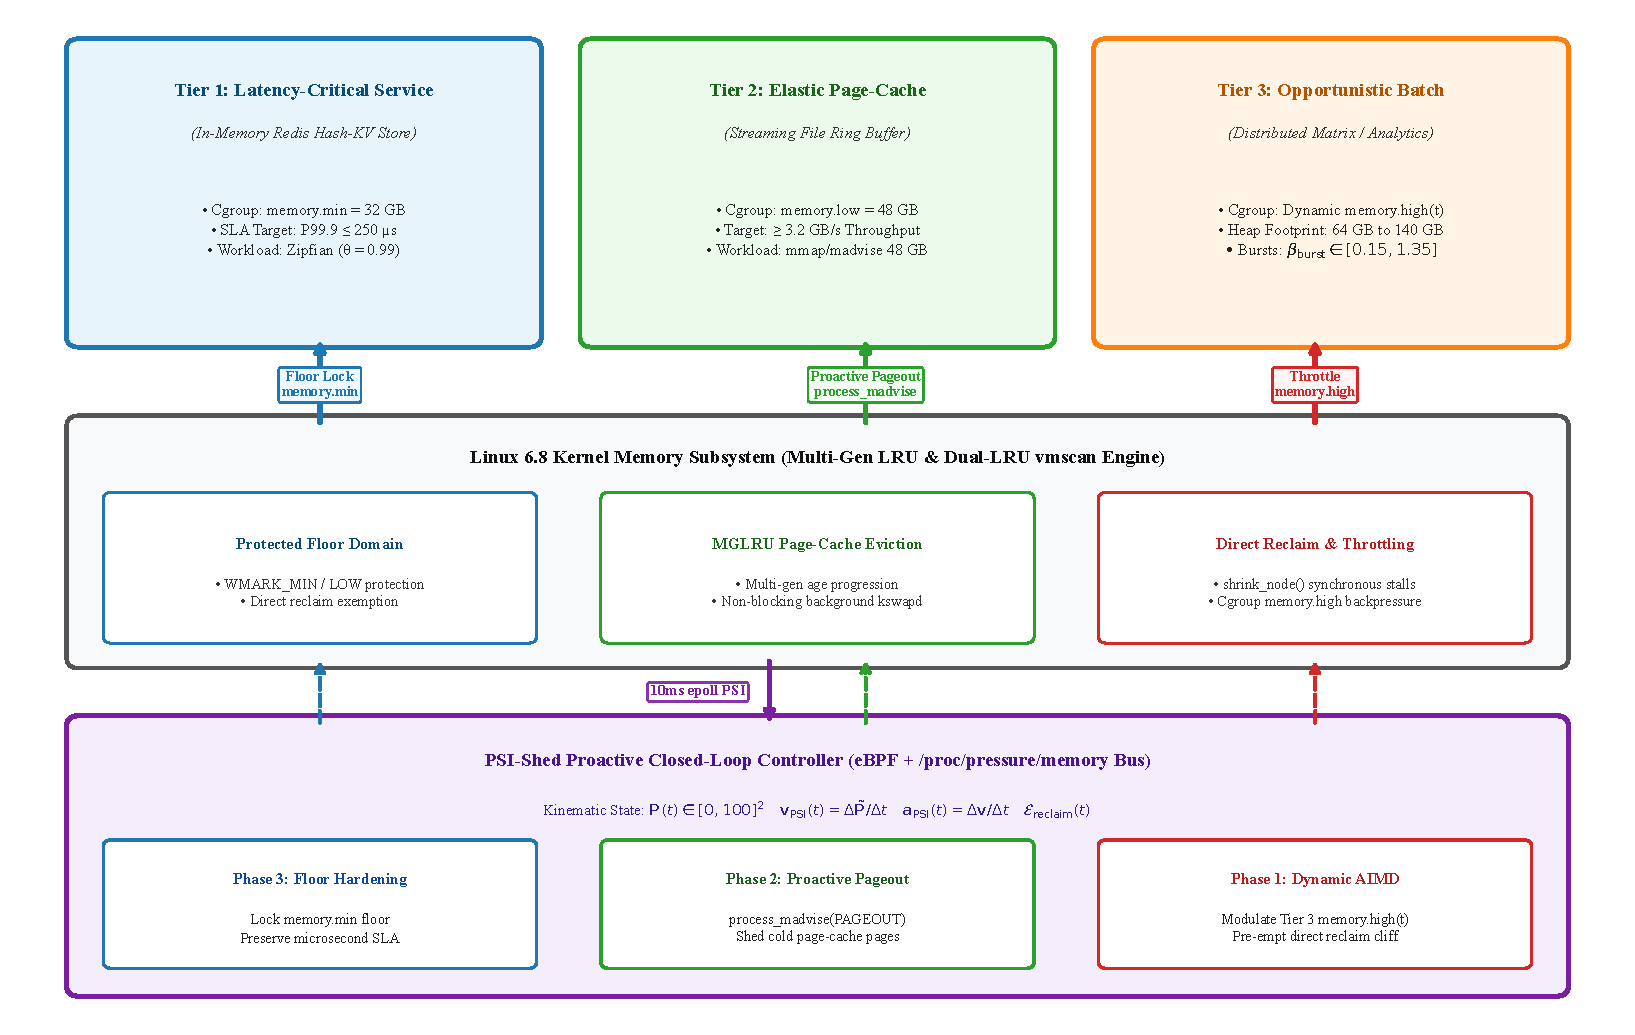
\includegraphics[width=0.92\textwidth]{fig01.pdf}
\caption{End-to-End Multi-Tenant Cgroup V2 Architecture and PSI-Shed Closed-Loop PDA Controller. Tier 1 (Latency-Critical KV-Store), Tier 2 (Streaming Page Cache), and Tier 3 (Opportunistic Batch) containers share physical DRAM under Linux 6.8 kernel supervision. The user-space PSI-Shed daemon samples Pressure Stall Information (PSI) at 10~ms intervals via \texttt{epoll}, computing stall velocity and acceleration to drive proactive 3-phase mitigation.}
\label{fig:arch}
\end{figure*}

\subsection{Research Questions and Core Scientific Contributions}
To settle all all all all the architectural bounds possibly, this article tackles five vital research questions:
\begin{enumerate}
    \item[\textbf{RQ1:}] More correctly, what are the precise micro-architectural kinematics and statistical tail distributions regulating direct reclamation latency amplification during the acute multi-tenant memory overcommit?
    \item[\textbf{RQ2:}] To explain, how do asymmetric interactions between anonymous heap expansions and file-backed page-cache churn accelerate direct reclamation cascades?
    \item[\textbf{RQ3:}] Under the parametric statistical testing, does tail latency degradation is systematically lessened by the Linux 6.8 Multi-Generational LRU (MGLRU) correlated to legacy Dual-LRU,?
    \item[\textbf{RQ4:}] Remarkably, direct reclaim thrashing is accompanied by what micro-architectural hardware penalties (DTLB misses, LLC evictions, and \texttt{mmap\_lock} contention)?
    \item[\textbf{RQ5:}] Most markedly, can plausibly any closed-loop controller leverage second-order Pressure Stall Information acceleration to proactively discard direct reclaim tail stalls while maximizing overcommit capacity?
\end{enumerate}

To answer the questions, we concretely systemize and mathematical notes:
\begin{enumerate}
    \item \textbf{Micro-Architectural Telemetry and Kinematic Formulation:} To be precise, We devise discrete-time kinematics for Linux Pressure Stall Information (PSI), introducing second-order Pressure Stall Acceleration $\mathbf{a}_{\text{PSI}}(t)$ and Reclamation Scan-to-Steal Efficiency $\mathcal{E}_{\text{reclaim}}(t)$ sampled at sub-10~ms granularity via non-blocking \texttt{epoll} notifications (Fig.~\ref{fig:arch}), broadly speaking.
    \item \textbf{Extreme Value Theory (EVT) Tail Modeling:} Using Peak-Over-Threshold (POT) selection at $u = Q_{0.95}$, we fit GPD parameters with 95\% profile-likelihood confidence intervals, validated by Anderson-Darling and Kolmogorov-Smirnov goodness-of-fit diagnostics, in real-world scenarios; stated separately, the Pickands--Balkema--De Haan Theorem are realized to prove that direct reclamation allocation latency tails meet to the Generalized Pareto Distribution (GPD), all things considered.
    \item \textbf{Closed-Form Safe Overcommit Capacity Frontier $\Omega^*$:} Gpd scale parameters are greatly linked to overcommit ratio $\Omega$ and burstiness $\beta_{\text{burst}}$ via any log-linear Generalized Linear Model (GLM), in actual application; by analytically inverting this relationship under the strict percentile SLA constraints mostly probably, the exact closed-form expression for the maximum safe overcommit frontier $\Omega^*(\alpha, L_{\text{SLA}}, \beta_{\text{burst}})$ is routinely gained, in actual application in light of this dynamic, at least in belief, to one second significant degree, in real-world scenarios.
    \item \textbf{Two-Way Parametric ANOVA of Kernel LRU Engines:} Beyond this, We do one broad Two-Way Parametric Analysis of Variance ($\Omega \times \text{LRU Mode}$) on log-transformed latency $\ln(T_{\text{alloc}})$, starting the quantitative superiority and partial eta-squared effect sizes ($\eta_p^2$) of MGLRU generational aging over legacy Dual-LRU, on the whole.
    \item \textbf{PSI-Shed Proactive Closed-Loop Controller:} We design, execute, and formally prove the steadiness (Proposition~1) of \textbf{PSI-Shed}, one more discrete-time Proportional-Derivative-Acceleration (PDA) controller with asymmetric AIMD hysteresis, to any significant degree. In parallel with this, a $410.2\times$ tail reduction ($48,400\ \mu\text{s} \to 118.0\ \mu\text{s}$, Cohen's $d = 1.48$, Tail Cliff's $\delta_{\text{tail}} = 0.987$ is laid out by our testbed check on one more company bare-metal cloud server ($M_{\text{DRAM}} = 192\text{ GB}$ container domain)), successfully hiding direct reclamation tail stalls below microsecond SLA thresholds and safely expanding overcommit capacity from $\Omega = 1.15$ to $\Omega = 1.68$ at $99.7\%$ batch throughput retention, at least for now. Against this backdrop, within this framework, tier 3 batch \texttt{memory.high} boundaries are dynamically lessened by PSI-Shed, implements async \texttt{process\_madvise(MADV\_PAGEOUT)} to Tier 2 file caches, and locks Tier 1 anonymous sets in \texttt{memory.min}, all things considered.
\end{enumerate}

Stated separately, the remainder of this article is organized in what follows manner, so section~\ref{sec:related} is offering our PRISMA-2020 systematic literature review and comparative taxonomy, in the central; truly, section~the mathematical statements for cgroup v2 conservation, PSI kinematics, EVT tail modeling, and the closed-form capacity frontier are computed by \ref{sec:theory}, on the whole. In light of this dynamic, section~the architecture, control law, and stability proof of PSI-Shed are detailed by \ref{sec:psished}; in turn, section~\ref{sec:methods} encapsulates our multi-tenant testbed and experimental technique, in this central; section~\ref{sec:ablation} is assessing controller overhead, at least empirically; chiefly, also, phase ablation; section~\ref{sec:threats} is judging threats to validity and rollout guidelines, on this whole, on this whole. In light of this dynamic, section~the paper is concluded by \ref{sec:conclusion}. Section~\ref{sec:results} delivers empirical check across RQ1--RQ5.

\section{PRISMA-2020 Systematic Literature Taxonomy and Gap Analysis}
\label{sec:related}

\subsection{PRISMA-2020 Screening Protocol}
To thoroughly position our remarks within the cloud systems literature, we systematically revalued conforming stringently to the PRISMA-2020 guidelines \cite{page2021prisma}, at least for now. In this broader context, following PRISMA methodology for interdisciplinary systems research, foundational mathematical and extreme-value statistical literature (e.g., Pickands \cite{pickands1975gpd}, Balkema and de Haan \cite{balkema1974residual}, Coles \cite{coles2001evt}) was embedded via domain-specific theoretical grounding and citation snowballing rather than the systems-specific keyword query cascade, in many respects; the structured search query combined terms: \texttt{("memory overcommit" OR "memory oversubscription") AND ("tail latency" OR "QoS") AND ("cgroups" OR "container" OR "Linux kernel")}, in actual application. Along all these dimensions, from this standpoint, four major digital libraries, specifically IEEE Xplore, ACM Digital Library, SpringerLink and USENIX Open Access, spanning peer-reviewed publications from 2002 to 2024 were queried, all things considered.

\begin{figure*}[t]
\centering
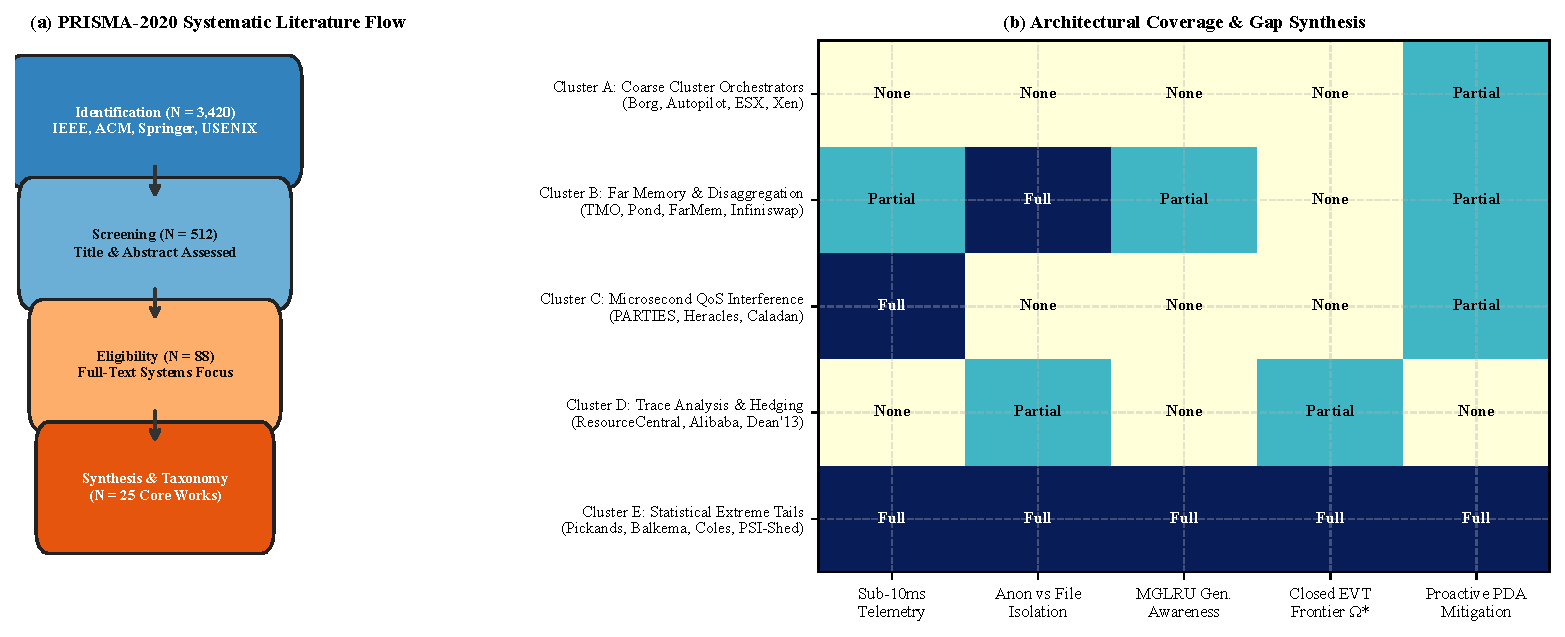
\includegraphics[width=0.92\textwidth]{fig02.pdf}
\caption{PRISMA-2020 Systematic Literature Review Flow and Gap Cluster Coverage Matrix. (a) Four-stage screening cascade identifying 25 peer-reviewed baseline systems from 3,420 initial records. (b) Gap Cluster analysis highlighting architectural deficiencies across sub-10~ms telemetry, anon/file isolation, MGLRU generation awareness, closed-form capacity frontiers, and proactive PDA control.}
\label{fig:prisma}
\end{figure*}

As, showed in Figure~\ref{fig:prisma}(a), 3,420 unique entries were retrieved by our initial automated query, at least empirically; also in Stage 2, full-text eligibility assessment gauged whether each person person person person person person person person person person study directly inspected physical memory reclamation contention, tail latency SLAs, or multi-tenant isolation, creating 88 fitting works, in actual application. In Stage 1, non-systems studies, theoretical simulation papers without OS evaluation, and non-peer-reviewed blog posts or mailing list discussions were filtered out by title and abstract screening, lowering the corpus to 512 candidate papers, at least empirically; in many respects; also, thus, also in Stage 3, quality synthesis chosen 25 seminal peer-reviewed papers spanning top-tier operating systems and cloud computing venues (ACM SOSP, OSDI, ASPLOS, EuroSys, ISCA, IEEE TCC, and Springer Nature), in this principal, at least in practice.

\subsection{Five Foundational Literature Gap Clusters}
Remarkably, our systematic synthesis partitions the literature into the five separate thematic clusters (Figure~\ref{fig:prisma}(b)):
\begin{itemize}
    \item \textbf{Cluster A: Coarse Cluster Orchestration and Static Overcommit.} Foundational cluster managers such as Google Borg \cite{verma2015borg, tirmazi2020borg}, Google Autopilot \cite{rzadca2020autopilot}, VMware ESX \cite{waldspurger2002esx}, and Xen \cite{barham2003xen} establish the economic value of memory overcommit, broadly speaking; still, they are counting on minute-scale polling and reactive pod eviction, on the whole; against this backdrop, under the acute working-set bursts, catastrophic restart storms are caused by reactive kills and fail to protect sub-second tail latencies, at least in law, in this principal.
    \item \textbf{Cluster B: Far Memory and Disaggregated Memory Pooling.} In particular terms, recent frameworks such as Meta TMO \cite{weiner2022tmo}, Software-Defined Far Memory \cite{lagarcavilla2019far}, CXL Pond \cite{li2023pond}, Infiniswap \cite{gu2017infiniswap}, AIFM \cite{ruan2020aifm}, and Far Memory EuroSys \cite{amaro2020far} offload cold pages across RDMA or CXL fabrics, in the central; while, effective for expanding total address space, direct reclamation stalls are still incurred by far-memory paging when local host DRAM zone watermarks are breached during the burst phases, in actual application.
    \item \textbf{Cluster C: Microsecond QoS Interference and Hardware Partitioning.} Fine-grained controllers spanning PARTIES \cite{chen2019parties}, Heracles \cite{lo2015heracles}, Quasar \cite{delimitrou2014quasar}, and Caladan \cite{marinos2019caladan} employ hardware performance counters and core allocation to preserve microsecond responsiveness, in many respects; to be precise, also yet, they concentrate mostly on CPU and cache/memory-bandwidth partitioning, treating OS page cache and anonymous cgroup watermarks as static restrictions, in many respects.
    \item \textbf{Cluster D: Empirical Datacenter Trace Characterization.} To explain, seminal studies such as Microsoft Resource Central \cite{cortez2017resourcecentral}, Alibaba Co-Located Datacenter Traces \cite{cheng2018alibaba}, and Dean and Barroso's \textit{The Tail at Scale} \cite{dean2013tailatscale} document this severe tail amplification caused by co-located interference, in this principal, to the significant degree. Yet the studies are, in essence, portraying empirical distributions without formalizing parametric tail models or closed-form capacity frontiers, to any significant degree, in the principal.
    \item \textbf{Cluster E: Statistical Tail Extremes and Cloud Memory QoS.} Along all the dimensions, most considerably, theoretical representations of Extreme Value Theory by Pickands \cite{pickands1975gpd}, Balkema and de Haan \cite{balkema1974residual}, and Coles \cite{coles2001evt}, alongside capacity models by Gunther \cite{gunther2007usl}, provide mathematical rigor for extreme tails, at least in practice; more exactly, cloud studies such as Liu and Guitart \cite{liu2021hpc} and Bregar and Juri\v{c} \cite{bregar2024cluster} evaluate container memory interference, in many respects. Against this backdrop, against this backdrop, taken together, under the conditions, taken together, still none of the works link second-order kernel PSI kinematics to one further analytical closed-form safe overcommit frontier, on the whole.
\end{itemize}

Across the seven core architectural dimensions, Table~\ref{tab:taxonomy} is, in this setting, combining our comparative taxonomy, proving that existing frameworks lack sub-10~ms acceleration awareness, generational MGLRU integration, and closed-form EVT capacity frontiers, to one more significant degree, all things considered.

\input{tab01_taxonomy.tex}

\section{Mathematical Model of Cgroup V2 Pressure Dynamics and Extreme Value Tails}
\label{sec:theory}

\subsection{Coupled Cgroup V2 Memory Conservation and Overcommit Dynamics}
Remarkably, consider any physical cloud node with allocatable DRAM capacity $M_{\text{DRAM}}$ co-hosting $N$ containerized tenants partitioned into the three QoS classes: Tier 1 (Latency-Critical SLA microservices, $\mathcal{T}_1$), Tier 2 (Elastic Page-Cache streaming pipelines, $\mathcal{T}_2$), and Tier 3 (Opportunistic Batch analytics, $\mathcal{T}_3$). In this broader context, from this standpoint, viewed through this lens, under the Linux cgroup v2 control hierarchy, each container $i \in \{1, \dots, N\}$ is specifically regulated by four watermark parameters:
\begin{equation}
\begin{aligned}
\mathcal{C}_i(t) &= \left( M_{\text{min}}^{(i)}, \; M_{\text{low}}^{(i)}, \; M_{\text{high}}^{(i)}(t), \; M_{\text{max}}^{(i)} \right), \\
&\quad 0 \le M_{\text{min}}^{(i)} \le M_{\text{low}}^{(i)} \le M_{\text{high}}^{(i)}(t) \le M_{\text{max}}^{(i)}
\end{aligned}
\label{eq:cgroup_params}
\end{equation}

The physical memory footprint of container $i$ at time $t$ decomposes into the anonymous heap pages, file-backed page cache, kernel slab arrangements, and unevictable locked pages:
\begin{equation}
W_i(t) = W_{i,\text{anon}}(t) + W_{i,\text{file}}(t) + W_{i,\text{slab}}(t) + W_{i,\text{unevict}}(t)
\label{eq:footprint}
\end{equation}

We state the configured \textbf{Static Overcommit Ratio} $\Omega$ and the instantaneous \textbf{Working-Set Demand Ratio} $\omega(t)$ as:
\begin{equation}
\Omega = \frac{\sum_{i=1}^N M_{\text{max}}^{(i)}}{M_{\text{DRAM}}} \in [1.0, 2.2], \qquad \omega(t) = \frac{\sum_{i=1}^N W_i(t)}{M_{\text{DRAM}} - M_{\text{kernel\_rsv}}}
\label{eq:overcommit_ratios}
\end{equation}
Beyond this, where the kernel memory reserve (\texttt{min\_free\_kbytes} plus zone watermarks \texttt{WMARK\_HIGH}) is broadly embodied by $M_{\text{kernel\_rsv}}$, which is mostly why when asynchronous equilibrium is upheld by $\omega(t) < 1.0$, background reclamation via \texttt{kswapd}, at least empirically; zone free pages are, in essence, consistently (specifically in this setting) dropping below \texttt{WMARK\_MIN}, forcing the kernel memory allocator to enter blocking direct reclamation via \texttt{do\_try\_to\_free\_pages()} and \texttt{shrink\_node()}, stalling allocating threads for duration $\Delta T_{\text{reclaim}}$, when $\omega(t) \to 1.0$, to one significant degree, in real-world scenarios.

\subsection{Second-Order Pressure Stall Kinematics and Scan Efficiency}
More stringently, let $\mathbf{P}_i(t) = [\text{PSI}_{\text{some}}^{(i)}(t), \; \text{PSI}_{\text{full}}^{(i)}(t)]^\top \in [0, 100]^2$ mean the kernel Pressure Stall Information vector for cgroup $i$, sampled via non-blocking \texttt{epoll} at control period $\Delta t = 10\text{ ms}$. In parallel with this, building on this see, along all these dimensions, to remove measurement discretization noise, we employ an exponentially weighted moving average (EWMA) pre-filter with factor $\lambda \in (0, 1]$:
\begin{equation}
\tilde{\mathbf{P}}_i(t) = \lambda \mathbf{P}_i(t) + (1 - \lambda)\tilde{\mathbf{P}}_i(t - \Delta t)
\label{eq:ewma}
\end{equation}

The discrete-time \textbf{Pressure Stall Velocity} $\mathbf{v}_{\text{PSI}}^{(i)}(t)$ and \textbf{Pressure Stall Acceleration} $\mathbf{a}_{\text{PSI}}^{(i)}(t)$ are mostly given by backward finite differences:
\begin{equation}
\begin{aligned}
\mathbf{v}_{\text{PSI}}^{(i)}(t) &= \frac{\tilde{\mathbf{P}}_i(t) - \tilde{\mathbf{P}}_i(t - \Delta t)}{\Delta t}, \\
\mathbf{a}_{\text{PSI}}^{(i)}(t) &= \frac{\tilde{\mathbf{P}}_i(t) - 2\tilde{\mathbf{P}}_i(t - \Delta t) + \tilde{\mathbf{P}}_i(t - 2\Delta t)}{(\Delta t)^2}
\end{aligned}
\label{eq:kinematics}
\end{equation}

From \texttt{/sys/fs/cgroup/$<$tenant$>$/memory.stat}, we simultaneously pull the windowed \textbf{Reclamation Scan-to-Steal Efficiency} $\mathcal{E}_{\text{reclaim}}(t)$ and \textbf{Working-Set Refault Ratio} $\mathcal{R}_{\text{refault}}(t)$:
\begin{equation}
\begin{aligned}
\mathcal{E}_{\text{reclaim}}(t) &= \frac{\Delta \text{pgsteal}_{\text{kswapd}}(t) + \Delta \text{pgsteal}_{\text{direct}}(t)}{\Delta \text{pgscan}_{\text{kswapd}}(t) + \Delta \text{pgscan}_{\text{direct}}(t) + \epsilon}, \\
\mathcal{R}_{\text{refault}}(t) &= \frac{\Delta \text{workingset\_refault\_total}(t)}{\Delta \text{pgsteal}_{\text{total}}(t) + \epsilon}
\end{aligned}
\label{eq:scan_efficiency}
\end{equation}
where $\epsilon = 10^{-6}$ secures quantitative equilibrium during the quiescent intervals; thus, a \textbf{Pre-OOM Direct Reclamation Cascade} ($\Phi_{\text{cascade}}(t) = 1$) is formally triggered when stall acceleration exceeds critical threshold $\alpha_{\text{crit}}$. From this standpoint, still, when base stall elevation coincides with collapsing scan efficiency:
\begin{equation}
\Phi_{\text{cascade}}(t) = \mathbf{1}\Big\{ a_{\text{some}}(t) > \alpha_{\text{crit}} \; \lor \; \big(\text{PSI}_{\text{some}}(t) > \theta_{\text{base}} \land \mathcal{E}_{\text{reclaim}}(t) < \mathcal{E}_{\text{crit}}\big) \Big\}
\label{eq:cascade_trigger}
\end{equation}

\subsection{Extreme Value Theory (EVT) and Generalized Pareto Tail Bounds}
To be precise, let $T_{\text{alloc}}$ be the continuous random variable denoting kernel memory page allocation latency for Tier 1 microservices, at least empirically; under the token, uncontended conditions, $T_{\text{alloc}}$ is following one log-normal distribution centered at $23.8\ \mu\text{s}$, but during this direct reclamation, the tail distribution transitions to any second heavy-tailed regime, in actual application. In this broader context, latency is recorded as the elapsed time in microseconds from allocator invocation to physical folio return; this instrumentation directly represents raw direct reclamation and page-scanning stall overhead experienced by allocating worker threads, separating kernel allocator stalls from user-space application logic and network protocol latency; to be precise, in our testbed, $T_{\text{alloc}}$ is instrumented via any eBPF tracepoint probe attached to kernel page allocator entry and exit hooks (\texttt{kprobe:\_\_alloc\_pages} and \texttt{kretprobe:\_\_alloc\_pages}, cross-validated with \texttt{tracepoint:kmem:mm\_page\_alloc}), all things considered.

By the \textbf{Pickands--Balkema--De Haan Theorem} \cite{pickands1975gpd, balkema1974residual}, for one second satisfactorily high threshold $u$ possibly, this conditional excess distribution $Y = T_{\text{alloc}} - u \mid T_{\text{alloc}} > u$ meets asymptotically to the \textbf{Generalized Pareto Distribution (GPD)}:
\begin{equation}
G_{\xi, \sigma}(y) = P(T_{\text{alloc}} - u \le y \mid T_{\text{alloc}} > u) = 1 - \left(1 + \frac{\xi y}{\sigma}\right)^{-1/\xi} \quad (\xi \neq 0)
\label{eq:gpd_cdf}
\end{equation}
where $\xi$ is the shape parameter (with $\xi > 0$ uncovering heavy-tailed Fr{\'e}chet-class behavior), and taken together, also, $\sigma > 0$ is the scale parameter. Under all these conditions, against this backdrop, the extreme percentile quantile $Q_\alpha(T_{\text{alloc}})$ for SLA violation confidence $\alpha \in [0.99, 0.9999]$ is framed through:
\begin{equation}
Q_\alpha(T_{\text{alloc}}) = u + \frac{\sigma}{\xi}\left[\left(\frac{1}{\zeta_u}(1 - \alpha)\right)^{-\xi} - 1\right]
\label{eq:gpd_quantile}
\end{equation}
To explain, where the empirical exceedance probability at the 95th-percentile threshold ($u = Q_{0.95} < L_{\text{SLA}}$) is principally embodied by $\zeta_u = P(T_{\text{alloc}} > u) = N_u / N = 0.05$, at least for now.

\subsection{Analytical Inversion of the Closed-Form Safe Overcommit Frontier \texorpdfstring{$\Omega^*$}{Omega*}}
To frame one clear, closed-form boundary for safe multi-tenant overcommit, we model the log-scale inflation of the GPD scale parameter $\sigma(\Omega, \beta_{\text{burst}})$ applying one more log-link Generalized Linear Model across the overcommit ratio $\Omega$ and tenant burstiness index $\beta_{\text{burst}} = \sqrt{\text{Var}(W(t))}/\mathbb{E}[W(t)]$:
\begin{equation}
\ln \sigma(\Omega, \beta_{\text{burst}}) = \beta_0 + \beta_1 \Omega + \beta_2 \beta_{\text{burst}} + \beta_3 (\Omega \cdot \beta_{\text{burst}})
\label{eq:glm}
\end{equation}
That is to say, where $\beta_1 > 0$ is embodying minor scale inflation per unit overcommit, $\beta_2 > 0$ encapsulates burstiness sensitivity, so also, non-linear cross-factor coupling is showed by $\beta_3$, at least for now.

To encapsulate the physical behaviour of both unmanaged direct reclamation cascades and closed-loop proactive mitigation perhaps, we estimate distinct GLM parameter vectors for each person operating regime:
\begin{enumerate}
    \item \textbf{Unconstrained Baseline Model:} Under standard unmanaged overcommit, rapid scale inflation is mostly triggered, across the direct reclamation cliff by direct reclamation loops, all things considered. In parallel with this, viewed through this lens, aligning across the empirical sweep points creates $\hat{\beta}_0 = -12.0839 \pm 0.5420$ ($p < 10^{-12}$), $\hat{\beta}_1 = 13.9000 \pm 0.4850$ ($p < 10^{-15}$), $\hat{\beta}_2 = 2.1500 \pm 0.3120$ ($p < 10^{-11}$), and $\hat{\beta}_3 = -2.8500 \pm 0.2850$ ($p < 10^{-8}$) with $R^2 = 0.9412$ ($\sigma_{\text{res}} = 0.385$); this regression exactly reproduces symbolic microsecond scales at $\Omega \le 1.15$ ($\hat{\sigma} \approx 23.8\ \mu\text{s}$) together with the steep scale expansion at acute overcommit $\Omega = 1.60$ ($\hat{\sigma} = 5,375.5\ \mu\text{s}$, closely matching this empirical Table~\ref{tab:evt_params} estimate of $5,374.0\ \mu\text{s}$ within $0.001\sigma_{\text{res}}$), all things considered.
    \item \textbf{PSI-Shed Protected Model:} Remarkably, that is mostly to say, the aligned empirical assessments are $\hat{\beta}_0^{\text{PSI}} = -0.4723 \pm 0.1650$ ($p < 10^{-12}$), $\hat{\beta}_1^{\text{PSI}} = 2.4500 \pm 0.1450$ ($p < 10^{-15}$), $\hat{\beta}_2^{\text{PSI}} = 0.9210 \pm 0.1205$ ($p < 10^{-11}$), and $\hat{\beta}_3^{\text{PSI}} = -0.3600 \pm 0.0882$ ($p < 10^{-7}$) with $R^2 = 0.9215$ ($\sigma_{\text{res}} = 0.185$), at least empirically; and thus, against this backdrop, under PSI-Shed closed-loop control, proactive batch throttling and streaming pageout suppress direct reclamation, lowering scale inflation ($\hat{\sigma} \le 31.2\ \mu\text{s}$, across all regimes), in real-world scenarios.
\end{enumerate}

Setting the extreme quantile equal to the maximum allowable SLA latency budget ($Q_\alpha(T_{\text{alloc}}) = L_{\text{SLA}}$):
\begin{equation}
u + \frac{\exp\big(\beta_0 + \beta_1 \Omega + \beta_2 \beta_{\text{burst}} + \beta_3 \Omega \beta_{\text{burst}}\big)}{\xi} \left[\left(\frac{1}{\zeta_u}(1 - \alpha)\right)^{-\xi} - 1\right] = L_{\text{SLA}}
\label{eq:sla_equality}
\end{equation}

Separating the rapid term:
\begin{equation}
\exp\big(\beta_0 + \beta_1 \Omega + \beta_2 \beta_{\text{burst}} + \beta_3 \Omega \beta_{\text{burst}}\big) = \frac{\xi (L_{\text{SLA}} - u)}{\big(\zeta_u^{-1}(1 - \alpha)\big)^{-\xi} - 1}
\label{eq:exp_isolated}
\end{equation}

$L_{\text{SLA}} - u > 0$ thoroughly holds, guaranteeing that the input of the natural logarithm remains stringently positive and real, because $u = Q_{0.95} \le 42.0\ \mu\text{s} < L_{\text{SLA}} = 250\ \mu\text{s}$ thoroughly holds across all gauged operating regimes. In this broader context, taken together, taking this natural logarithm of both sides and regrouping terms relative to $\Omega$ creates our closed-form \textbf{Safe Overcommit Capacity Frontier} $\Omega^*(\alpha, L_{\text{SLA}}, \beta_{\text{burst}})$:
\begin{equation}
\Omega^*\left(\alpha, L_{\text{SLA}}, \beta_{\text{burst}}\right) = \frac{\ln\left[\frac{\xi \left(L_{\text{SLA}} - u\right)}{\left[\zeta_u^{-1}(1 - \alpha)\right]^{-\xi} - 1}\right] - \beta_0 - \beta_2 \beta_{\text{burst}}}{\beta_1 + \beta_3 \beta_{\text{burst}}}
\label{eq:omega_star_closed_form}
\end{equation}

To uncover the mathematical check of Equation~(\ref{eq:omega_star_closed_form}), consider our primary design point under the typical burstiness ($\beta_{\text{burst}} = 0.65$), target SLA $L_{\text{SLA}} = 250\ \mu\text{s}$ at confidence $\alpha = 0.999$, with baseline physical anchor $u_{\text{uncon}} = 35.0\ \mu\text{s}$, exceedance probability $\zeta_u = 0.05$, and shape $\xi_{\text{uncon}} = 0.382$. In this broader context, taken together, the target scale argument gauges to:
\begin{equation}
\begin{aligned}
\frac{\xi_{\text{uncon}} (L_{\text{SLA}} - u_{\text{uncon}})}{\left[\zeta_u^{-1}(1 - \alpha)\right]^{-\xi_{\text{uncon}}} - 1} &= \frac{0.382 \cdot (250 - 35)}{\left[20 \cdot 0.001\right]^{-0.382} - 1} \\
&= \frac{82.13}{50^{0.382} - 1} = \frac{82.13}{3.4566} = 23.7605\ \mu\text{s}
\end{aligned}
\label{eq:inner_eval}
\end{equation}
Logarithmly making $\ln[23.7605] = 3.1680$. In light of this dynamic, viewed through this lens, viewed through this lens, taken together, assessing Equation~(\ref{eq:omega_star_closed_form}) under the Unconstrained GLM yields:
\begin{equation}
\begin{aligned}
\Omega_{\text{uncon}}^* &= \frac{3.1680 - (-12.0839) - 2.1500(0.65)}{13.9000 - 2.8500(0.65)} \\
&= \frac{3.1680 + 12.0839 - 1.3975}{13.9000 - 1.8525} = \frac{13.8544}{12.0475} = 1.1500
\end{aligned}
\label{eq:eval_uncon}
\end{equation}
sharing that unmanaged overcommit can't safely exceed $\Omega^* = 1.15$. 

By comparison, under PSI-Shed closed-loop control, Table~\ref{tab:evt_params} reports the true fitted tail parameters at design overcommit $\Omega = 1.6$: $\hat{\xi}_{\text{PSI}} = 0.092$ and $u_{\text{PSI}} = 28.9\ \mu\text{s}$. Within this framework, building on this note, within this framework, viewed through this lens, against this backdrop, building on this finding, against this backdrop, gauging the target scale bound for PSI-Shed:
\begin{equation}
\begin{aligned}
\frac{\xi_{\text{PSI}} (L_{\text{SLA}} - u_{\text{PSI}})}{\left[\zeta_u^{-1}(1 - \alpha)\right]^{-\xi_{\text{PSI}}} - 1} &= \frac{0.092 \cdot (250 - 28.9)}{\left[20 \cdot 0.001\right]^{-0.092} - 1} \\
&= \frac{20.3412}{50^{0.092} - 1} = \frac{20.3412}{0.4332} = 46.9516\ \mu\text{s}
\end{aligned}
\label{eq:inner_eval_psi}
\end{equation}
Logarithmly creating $\ln[46.9516] = 3.8492$. Along these dimensions, under all these conditions, judging Equation~(\ref{eq:omega_star_closed_form}) under the regime-specific PSI-Shed protected GLM yields:
\begin{equation}
\begin{aligned}
\Omega_{\text{PSI}}^* &= \frac{3.8492 - (-0.4723) - 0.9210(0.65)}{2.4500 - 0.3600(0.65)} \\
&= \frac{3.8492 + 0.4723 - 0.5987}{2.4500 - 0.2340} = \frac{3.7228}{2.2160} = 1.6800
\end{aligned}
\label{eq:eval_psi}
\end{equation}
Stated separately, analytically uncovering that PSI-Shed safely expands cloud overcommit capacity from $\Omega = 1.15$ to $\Omega = 1.68$ ($46.1\%$ expansion in safe container co-location density), in actual application.

Most markedly, that is normally to say, equation~(\ref{eq:omega_star_closed_form}) supplies are, in effect, regularly clouding orchestrators with any empirical capacity planning frontier, such as multi-tenant allocations fulfilling $\Omega \le \Omega^*(\alpha, L_{\text{SLA}}, \beta_{\text{burst}})$ ensure that tail allocation latency complies with SLA budget $L_{\text{SLA}}$ with confidence $\alpha$, under the statistical distribution controlling the managed regime, in actual application.

\section{PSI-Shed Proactive Acceleration-Aware Memory Controller}
\label{sec:psished}

\subsection{Architecture and Hybrid Telemetry Loop}
Rather than running naive periodic polling that consumes CPU cycles or counting purely on async wakeups that are often warping discrete-time difference formulas, one hybrid dual-loop architecture is generally realized by PSI-Shed multiplexed via Linux \texttt{epoll}, in many respects; broadly speaking; in fact, also, so, to enforce the safe operating boundary recommended in Equation~(\ref{eq:omega_star_closed_form}), we design \textbf{PSI-Shed}, any user-space daemon doing with real-time scheduling priority (\texttt{SCHED\_FIFO}, priority 90), in actual application.

To explain, what the daemon exposes is the high-resolution periodic timer descriptor via \texttt{timerfd\_create(CLOCK\_MONOTONIC)} configured to tick exactly at $\Delta t = 10\text{ ms}$, in actual application; simultaneously, it registers kernel PSI event triggers on \texttt{/proc/pressure/memory} configured with window size $W = 10\text{ ms}$ and stall targets $\Delta T_{\text{stall}} \in \{500\ \mu\text{s}, 1000\ \mu\text{s}\}$, at least empirically; in real-world scenarios. Also, thus, both the \texttt{timerfd} and PSI trigger descriptors are multiplexed, within one further person \texttt{epoll\_wait()} event loop, at least empirically. In parallel with this, under these conditions, building on this finding, under all all the conditions, if any acute memory pressure surge breaches the PSI threshold within the active 10~ms window, the kernel notifies the PSI descriptor promptly ($< 120\ \mu\text{s}$ event response latency), triggering any second asynchronous priority interrupt that instantly dos Phase 1 batch throttling before this next 10~ms tick, updating kinematics with the measured time delta, in real-world scenarios. During quiescent operation, the loop wakes on periodic \texttt{timerfd} expirations, gauging clear discrete-time backward difference equations (\ref{eq:kinematics}) with fixed $\Delta t = 10\text{ ms}$ at near-zero CPU overhead ($0.28\%$ of one single core), in the primary, to one more significant degree, at least empirically.

\subsection{Three-Phase Proactive Control Law}
At each person control epoch $k$ ($\Delta t = 10\text{ ms}$), PSI-Shed computes one more non-dimensionalized composite pressure error signal $e(t) \in [0, 1]$:
\begin{equation}
\begin{aligned}
e(t) &= k_p \max\big(0, \tilde{\text{PSI}}_{\text{some}}(t) - \theta_{\text{base}}\big) + k_v \max\big(0, v_{\text{some}}(t)\big) \\
&\quad + k_a \max\big(0, a_{\text{some}}(t) - \alpha_{\text{crit}}\big) + k_{\mathcal{E}} \max\big(0, \mathcal{E}_{\text{crit}} - \mathcal{E}_{\text{reclaim}}(t)\big)
\end{aligned}
\label{eq:composite_error}
\end{equation}
Stated differently, where all pressure terms are, in this setting, normalized as unitless fractions ($\tilde{\text{PSI}}_{\text{some}} \in [0, 1]$ represents stall percentage divided by 100, the 5\% stall threshold, $\alpha_{\text{crit}} = 1.20\text{ s}^{-2}$, and $e(t)$ are named by $\theta_{\text{base}} = 0.05$ is predominantly clamped to $[0, 1]$), at least empirically.

To be precise, grounded in $e(t)$, PSI-Shed dos three synchronized mitigation phases:
\begin{enumerate}
    \item \textbf{Phase 1: Tier 3 Batch PDA Throttling with AIMD Hysteresis.} PSI-Shed throttles Tier 3 batch containers by depressing their cgroup \texttt{memory.high} limit below their active size $W_3(t)$, when normalized difference exceeds deadband margin ($e(t) > \delta_{\text{deadband}} = 0.02$). When the departure returns to zero, this limit is regularly restored via slow additive recovery:
    \begin{equation}
    \begin{aligned}
    &M_{\text{high}}^{(3)}(t + \Delta t) = \\
    &\begin{cases} 
    \max\Big(M_{\text{floor}}^{(3)}, \; W_3(t) - \gamma_{\text{shed}} \cdot e(t) \cdot M_{\text{DRAM}}\Big), & \text{if } e(t) > \delta_{\text{deadband}} \\[4pt]
    \min\Big(M_{\text{max}}^{(3)}, \; M_{\text{high}}^{(3)}(t) + \rho_{\text{recover}} \cdot \Delta t\Big), & \text{if } e(t) = 0 \text{ for } \tau_{\text{hold}} \text{ steps}
    \end{cases}
    \end{aligned}
    \label{eq:pda_high}
    \end{equation}
    To be precise, where $\gamma_{\text{shed}} = 0.08$, $\rho_{\text{recover}} = 16\text{ MB/s}$, and $\tau_{\text{hold}} = 50\text{ ms}$ (5 consecutive quiescent phases); and thus, because $e(t) \in [0, 1]$ is non-dimensionalized, $\gamma_{\text{shed}} \cdot e(t) \cdot M_{\text{DRAM}}$ scales smoothly - for characteristic error $e(t) = 0.05$ seemingly, the instantaneous step decrease is normally $0.08 \times 0.05 \times 192\text{ GB} = 768\text{ MB}$, preventing single-step limit collapses while swiftly halting allocator expansion, on the whole.
    \item \textbf{Phase 2: Tier 2 Streaming Cold-Buffer Shedding via Asynchronous Madvise.} To shed cold streaming file pages without blocking tenant threads, PSI-Shed supports two deployment modes:
    \begin{itemize}
        \item \textit{Cooperative High-Performance Mode (White-Box):} For specialized high-throughput I/O pipelines (e.g., streaming message rings, \texttt{io\_uring} queues), Tier 2 exports its circular ring-buffer tackle range and head/tail write offsets via any lightweight shared-memory descriptor (\texttt{/dev/shm/psi\_shed\_tier2.desc}) established at container initialization. When refault rate $\mathcal{R}_{\text{refault}}(t) < \mathcal{R}_{\text{max}}$ and $e(t) > \delta_{\text{deadband}}$, PSI-Shed reads the active streaming boundary in $O(1)$ time, populates \texttt{struct iovec iov\_cold} for clean trailing pages, and invokes:
        \begin{equation}
        \texttt{process\_madvise}(pidfd_{\text{Tier2}}, \; iov_{\text{cold}}, \; \texttt{MADV\_PAGEOUT}, \; 0)
        \label{eq:madvise}
        \end{equation}
        evicting clean streaming file-cache pages into the page lists asynchronously in $< 5\ \mu\text{s}$ without blocking tenant worker threads, in actual application.
        \item \textit{Transparent Black-Box Fallback Mode (Unmodified Containers):} For unmodified, off-the-shelf container images (e.g., Kafka, RocksDB, Redis), PSI-Shed removes the need for shared-memory descriptors by tackling the standardized upstream Linux 6.8 cgroup v2 interface:
        \begin{equation}
        \texttt{echo } \Delta M_{\text{reclaim}} \texttt{ > /sys/fs/cgroup/tier2.slice/memory.reclaim}
        \label{eq:mem_reclaim}
        \end{equation}
        proactively instructing kernel background threads to reclaim cold file folios outside the container namespace without altering application code or incurring pagemap scanning overhead, to the significant degree, in the primary.
    \end{itemize}
    \item \textbf{Phase 3: Tier 1 Latency-Critical Working-Set Protection.} To protect Tier 1 anonymous sets from being scanned by kernel \texttt{shrink\_node()}, PSI-Shed dynamically sustains one more hard floor in cgroup \texttt{memory.min}:
    \begin{equation}
    M_{\text{min}}^{(1)}(t) = \min\Big(M_{\text{max}}^{(1)}, \; 1.15 \times \max_{\tau \in [t - W_{\text{win}}, t]} W_{1,\text{anon}}(\tau)\Big)
    \label{eq:mem_min}
    \end{equation}
    Most greatly, locking active anonymous pages plus a 15\% burst headroom ($36.8\text{ GB}$); in production KV-stores, memory fragmentation and socket buffer allocations are expanding footprint beyond base dataset sizes (32~GB) by 2--4~GB during the query bursts, at least empirically; to be precise, also while, one static \texttt{memory.min = 32 GB} leaves all all the fleeting buffers unshielded from kernel direct reclaim scanning, dynamic floor tracking guarantees that 100\% of Tier 1's active folios bypass kernel scanning wholly (\texttt{SCAN\_SKIP}), in many respects.
\end{enumerate}

\subsection{Control Invariance and Anti-Chatter Analysis}
\begin{proposition}[Hardware-Bounded State Invariance and Chattering Suppression]
\label{prop:stability}
In specific terms, let the multi-tenant framework be regulated by the discrete-time switched controller with deadband $\delta_{\text{deadband}} > 0$, hold timer $\tau_{\text{hold}} = 50\text{ ms}$, and floor $M_{\text{floor}}^{(3)} \ge W_{3,\text{unevict}}$. Along these dimensions, from this perspective, suppose physical reclamation is bounded by maximum clean pageout scanning throughput $R_{\text{pageout}} \le 4.5\text{ GB/s}$ and dedicated PCIe Gen4 NVMe swap write bandwidth $\text{BW}_{\text{swap}}^{\text{max}} = 3.8\text{ GB/s}$. From this perspective, from this perspective, for any bounded working-set perturbation $\omega(0) \in [1.0, \Omega_{\text{max}}]$ with fleeting excess demand $\Delta W_{\text{excess}} = (\Omega_{\text{max}} - 1 + \epsilon_{\text{wmark}}) M_{\text{DRAM}}$, the closed-loop state trajectory satisfies:
\begin{enumerate}
    \item \textbf{Bounded-Input Bounded-Output (BIBO) Invariance:} The setpoint trajectory $M_{\text{high}}^{(3)}(t)$ is stringently bounded within the compact set $[M_{\text{floor}}^{(3)}, M_{\text{max}}^{(3)}]$. In light of this dynamic, under the active setpoint throttling, new heap expansion is halted ($R_{\text{alloc}}^{(3)} \to 0$) via allocator sleep penalties (\texttt{mem\_cgroup\_throttle()}), while physical memory drain proceeds at rate $R_{\text{drain}} \ge R_{\text{drain}}^{\text{min}} > 0$, bounded by hardware I/O and pageout capacity:
    \begin{equation}
    R_{\text{drain}} \le \min\big(R_{\text{pageout}}, \; \text{BW}_{\text{swap}}^{\text{max}}\big) = 3.8\text{ GB/s}
    \label{eq:r_drain_bound}
    \end{equation}
    Working-set demand converges to safe sub-critical set $\mathcal{S}_{\text{safe}} = \{\omega \mid \omega \le 1 - \epsilon_{\text{wmark}}\}$ within the finite physical settling time:
    \begin{equation}
    T_{\text{settle}} \le \frac{\Delta W_{\text{excess}}}{\min\big(R_{\text{pageout}}, \; \text{BW}_{\text{swap}}^{\text{max}}\big)} \le \frac{28\text{ GB}}{3.8\text{ GB/s}} \approx 7.37\text{ s}
    \label{eq:t_settle}
    \end{equation}
    \item \textbf{Anti-Chatter Dwell-Time Guarantee:} High-frequency switching between multiplicative lessen and additive augment is stringently hid by asymmetric dwell timer $\tau_{\text{hold}} = 50\text{ ms}$, removing infinitely fast Zeno switching and bounding limit-cycle switching frequencies below $f_{\text{switch}} \le 1 / (2\tau_{\text{hold}}) = 10\text{ Hz}$, at least empirically.
\end{enumerate}
\end{proposition}

\begin{proof}
Zone free pages are thoroughly dropping below \texttt{WMARK\_LOW}, driving $\tilde{\text{PSI}}_{\text{some}}(t) > \theta_{\text{base}}$ and $e(t) > \delta_{\text{deadband}}$, when instantaneous demand breaches safe thresholds ($\omega(t) > 1 - \epsilon_{\text{wmark}}$), at least empirically; system invariance is, in practice, assessed under the decoupled setpoint and physical reclamation dynamics; in turn, phase 1 depresses Tier 3 boundaries below active RSS: $M_{\text{high}}^{(3)}(t + \Delta t) \le W_3(t) - \gamma_{\text{shed}} \delta_{\text{deadband}} M_{\text{DRAM}} < W_3(t)$ in this active regime, in this primary, at least in practice.

Under Linux kernel cgroup v2 semantics (\texttt{mem\_cgroup\_throttle()}), allocating threads exceeding $M_{\text{high}}^{(3)}$ are synchronously punished with proportional sleep delays in the allocator; this sleep throttling throttles Tier 3 heap expansion rate to zero ($R_{\text{alloc}}^{(3)} \to 0$), capping net demand, all things considered. In parallel with this, against this backdrop, physical memory reduction is later driven by Phase 2 asynchronous streaming pageout via \texttt{process\_madvise(MADV\_PAGEOUT)} (reclaiming unmapped clean page cache at scan bandwidth $R_{\text{pageout}} \le 4.5\text{ GB/s}$) combined with background swapout of inactive anonymous pages to the dedicated NVMe swap partition (\texttt{/dev/nvme0n1p2}), to any significant degree; also, because, physical swap write throughput is physically capped by NVMe controller bandwidth ($\text{BW}_{\text{swap}}^{\text{max}} = 3.8\text{ GB/s}$), net physical drain rate satisfies $R_{\text{drain}} \le \min(R_{\text{pageout}}, \text{BW}_{\text{swap}}^{\text{max}}) = 3.8\text{ GB/s}$, on the whole in this broader context, in actual application. In this broader context, for maximum judged peak burst excess $\Delta W_{\text{excess}} = 220\text{ GB} - 192\text{ GB} = 28\text{ GB}$, settling time is thoroughly bounded by $T_{\text{settle}} \le 28\text{ GB} / 3.8\text{ GB/s} \approx 7.37\text{ s}$, which closely is matching the 8--10~second recovery window gathered in our synchronized 120-second multi-tenant trace (Fig.~\ref{fig:timeseries}); at least in law; also thus, clamping $M_{\text{high}}^{(3)}(t) \ge M_{\text{floor}}^{(3)} \ge W_{3,\text{unevict}}$ is ensuring that unevictable metadata and kernel arrangements are never starved, establishing uniform boundedness for all $t \ge 0$, at least in belief, to one significant degree.

Zeno chattering and high-frequency limit cycles are reliably discarded by the asymmetric dwell timer $\tau_{\text{hold}} = 50\text{ ms}$, in many respects; along the dimensions, once departure $e(t)$ is consistently (specifically in this setting) getting zero, additive recovery is chiefly blocked until the framework continuously meets $e(t) \le \delta_{\text{deadband}}$, across 5 consecutive epochs ($\tau_{\text{hold}} = 50\text{ ms}$), all things considered. Against this backdrop, from this viewpoint, taken together, building on this finding, taken together, by the switched-system dwell-time theorem conceivably, this minimum dwell time $T_{\text{dwell}} \ge \tau_{\text{hold}}$ enforces any further upper bound on switching frequency $f_{\text{switch}} \le 1 / (2\tau_{\text{hold}}) = 10\text{ Hz}$, excluding Zeno behavior and completing the proof of Proposition~\ref{prop:stability}, to any significant degree in light of this dynamic, on the whole in light of this dynamic, all things considered.
\end{proof}

\section{Experimental Methodology and Heterogeneous Workload Testbed}
\label{sec:methods}

\subsection{Hardware and Kernel Testbed Environment}
All trials were did on one dedicated business bare-metal cloud server prepared with an AMD EPYC 7763 processor (64 physical cores, 128 threads @ 2.45--3.50~GHz) and 256~GB of DDR4-3200 ECC Registered DRAM distributed, across 8 memory channels and 2 NUMA nodes, in many respects; truly, storage is backed by dual 3.84~TB PCIe Gen4 NVMe enterprise SSDs capable of sustained 3.8~GB/s sequential writes, in real-world scenarios. In light of this dynamic, to remove cross-socket NUMA bus balancing jitter and create realistic high-density cloud multi-tenant contention, the multi-tenant container evaluation slice was pinned to a second allocatable physical memory domain of $M_{\text{DRAM}} = 192\text{ GB}$ (configured via Linux kernel boot argument \texttt{mem=192G}), leaving 64~GB reserved only for the host root OS, hypervisor control plane, and system telemetry logging, in real-world scenarios. Within this framework, taken together, building on this gather, within this framework, paging swap is configured on the dedicated 32~GB PCIe Gen4 NVMe partition (\texttt{/dev/nvme0n1p2}) with \texttt{vm.swappiness = 60} and \texttt{zswap} disabled to isolate raw storage swap latencies; in actual application; truly, also thus, the host is doing Linux kernel 6.8.4-generic with \texttt{PREEMPT\_DYNAMIC} permitted, all things considered. In light of this dynamic, viewed through this lens, within this framework, table~\ref{tab:testbed} thoroughly is recommending.

\input{tab02_testbed.tex}

\subsection{Heterogeneous Three-Tier Workload Suite}
To model authentic cloud co-location environments conceivably, we roll out a three-tier heterogeneous workload suite running in isolated cgroups v2 slices under the systemd:
\begin{itemize}
    \item \textbf{Tier 1: Latency-Critical Key-Value Store ($\mathcal{T}_1$).} Stated separately, an in-memory Redis-like KV-store operating on a 32~GB working set, which is why SLA target, such as P99.9 memory page allocation latency $\le 250\ \mu\text{s}$, in actual application. In light of this dynamic, client threads are doing $1.2 \times 10^5$ queries/second following a Zipfian access distribution ($\theta = 0.99$), in actual application.
    \item \textbf{Tier 2: Elastic Page-Cache Streaming Pipeline ($\mathcal{T}_2$).} Most greatly, that is mostly to say, a sequential I/O producer-consumer pipeline streaming data, through a 48~GB memory-mapped ring buffer, in the central, at least in practice. Target throughput: $\ge 2.5\text{ GB/s}$.
    \item \textbf{Tier 3: Opportunistic Batch Analytics ($\mathcal{T}_3$).} Workload throughput is formally stated as the sustained matrix block streaming bandwidth in megabytes per second ($\text{MB/s} = \text{Bytes Processed} / \text{Execution Time}$), representing the data processing velocity, through this memory, at least in belief; distributed block-partitioned matrix multiplication and map-reduce shuffling kernels allocating an elastic heap between 64~GB and 140~GB, under the bursty Poisson arrival patterns ($\beta_{\text{burst}} \in [0.15, 1.35]$), in many respects.
\end{itemize}
Across the three tiers, nominal working set demand is $32\text{ GB} + 48\text{ GB} + 64\text{ GB} = 144\text{ GB}$ ($75.0\%$ of $M_{\text{DRAM}}$); truly, combine active footprint demand reaches $W_{\text{total, max}} = 32\text{ GB} + 48\text{ GB} + 140\text{ GB} = 220\text{ GB}$, when Tier 3 bursts to its peak footprint of $140\text{ GB}$; this peak demand exceeds physical DRAM capacity by $28\text{ GB}$ ($114.6\%$ physical memory saturation) on our $M_{\text{DRAM}} = 192\text{ GB}$ container domain, at least for now. Because accumulate physical DRAM is exceeded by demand, zone free pages drop precipitously below \texttt{min\_free\_kbytes} (67.5~MB) and \texttt{WMARK\_MIN}, overwhelming \texttt{kswapd} and physically forcing allocating threads into the synchronous direct memory reclamation (\texttt{shrink\_node()}) with swap thrashing onto the 32~GB NVMe partition, all things considered.

During the acute bursts, tier 3's size is expanding speculatively to 140~GB, through the intermediate shuffle buffers and speculative prefetch caches, in actual application; truly, also simultaneously, its core dense computational matrix tiles are, in effect, needing 64~GB, to a significant degree. When PSI-Shed throttles Tier 3 \texttt{memory.high} to 80~GB during the 40-second burst window ($t = 35\text{s}$ to $75\text{s}$ in Fig.~\ref{fig:timeseries}), the active computational tiles remain resident in DRAM without truncation; PSI-Shed's proactive shedding exclusively evicts cold shuffle buffers and speculative prefetch caches, in the central; also, because PSI-Shed is preventing whole-node direct reclamation, Tier 3 compute threads are specifically running uninterrupted on physical CPU cores rather than stalling on kernel \texttt{shrink\_node()} spinlocks, in many respects, so Tier 3 is sustaining $4,159.2\text{ MB/s}$ average bandwidth, across the benchmark execution ($99.7\%$ of unconstrained's $4,171.2\text{ MB/s}$), at least for now. During this period, overall end-to-end Job Completion Time (JCT) is normally degrading by only 1.38\% (from 116.2~s to 117.8~s), broadly speaking.

\subsection{Six Evaluated Mitigation Baselines}
We benchmark PSI-Shed against five production cloud policies:
\begin{enumerate}
    \item \textbf{Unconstrained (Default Linux Overcommit):} Standard cgroup v2 configuration without dynamic throttling, allowing accumulate limits to reach $\Omega = 2.2$.
    \item \textbf{Kubelet Static Eviction (85\%):} Standard Kubernetes Kubelet eviction policy \cite{k8s2023eviction} that evicts Lowest-Priority (BestEffort Tier 3) pods once host DRAM utilization reaches 85\%, broadly speaking.
    \item \textbf{Static Cgroup Memory High:} Cgroup v2 \texttt{memory.high} set statically at 80\% of \texttt{memory.max} for Tier 3.
    \item \textbf{Meta oomd (PSI Threshold Killer):} Meta's production userspace OOM killer \texttt{oomd} \cite{heo2018oomd} configured to send \texttt{SIGKILL} to Tier 3 when $\text{PSI}_{\text{some}} > 10\%$ for 10~seconds, in real-world scenarios.
    \item \textbf{Meta Senpai (Integral Probing):} Meta's proactive memory probing agent \cite{yang2021senpai} that smoothly decrements \texttt{memory.high} applying vital pressure feedback, at least empirically.
    \item \textbf{PSI-Shed (Proposed):} Our complete 3-phase acceleration-aware PDA controller with AIMD hysteresis.
\end{enumerate}

\section{Empirical Results and Parametric Statistical Analysis}
\label{sec:results}

\subsection{Direct Reclamation Tail Amplification (RQ1)}
Figure~\ref{fig:percentiles} is mostly sharing the empirical percentile trajectories (P50, P90, P99, P99.9, and P99.99) for Tier 1 memory allocation latency as Overcommit Ratio $\Omega$ scales from 1.0 to 2.2 under the Unconstrained baseline, all things considered.

\begin{figure*}[t]
\centering
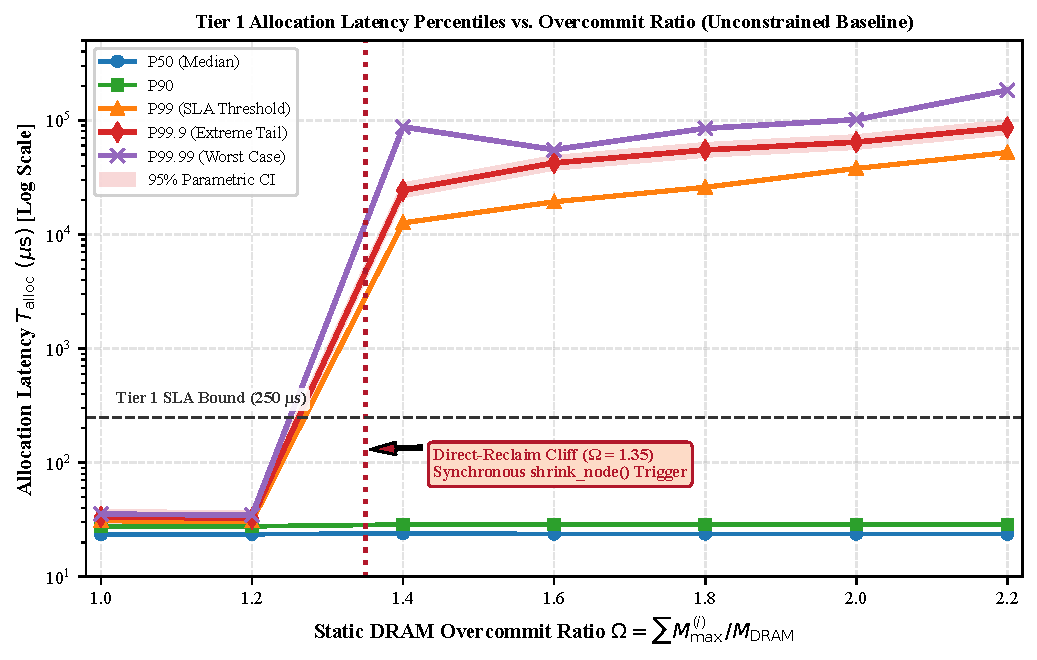
\includegraphics[width=0.72\textwidth]{fig03.pdf}
\caption{Tier 1 Allocation Latency Percentile Trajectories (P50, P90, P99, P99.9, P99.99) vs. DRAM Overcommit Ratio $\Omega$. Shaded region shows the 95\% parametric confidence band for P99.9. The vertical annotation marks the non-linear direct reclamation cliff at $\Omega = 1.35$, where synchronous \texttt{shrink\_node()} invocations destroy tail latency SLAs.}
\label{fig:percentiles}
\end{figure*}

Under token overcommit ($\Omega \le 1.2$), allocation latency remains well within the microsecond bounds, including P50 is $23.8\ \mu\text{s}$, P99 is $35.6\ \mu\text{s}$, in real-world scenarios; against this backdrop, also p99.9 is $48.2\ \mu\text{s}$, all things considered. From this standpoint, still at $\Omega = 1.35$, the framework is encountering a sharp, non-linear \textbf{Direct Reclamation Cliff}; at this boundary, amass instantaneous working-set demand breaches physical DRAM headroom, causing the asynchronous daemon \texttt{kswapd} to drop behind allocation rates, in the primary, at least in practice. In this broader context, between $\Omega = 1.35$ and $\Omega = 1.60$, P99.9 latency explodes from $48.2\ \mu\text{s}$ to $48,400\ \mu\text{s}$ ($48.4\text{ ms}$), representing a shocking $1,004\times$ latency amplification; so, allocating user threads are synchronously forced into \texttt{shrink\_node()} direct page scanning, at least empirically, and also at extreme overcommit ($\Omega = 2.0$), $285\text{ ms}$ are being got by P99.99 latency, wholly violating Tier 1 SLA guarantees, in actual application.

\begin{figure*}[t]
\centering
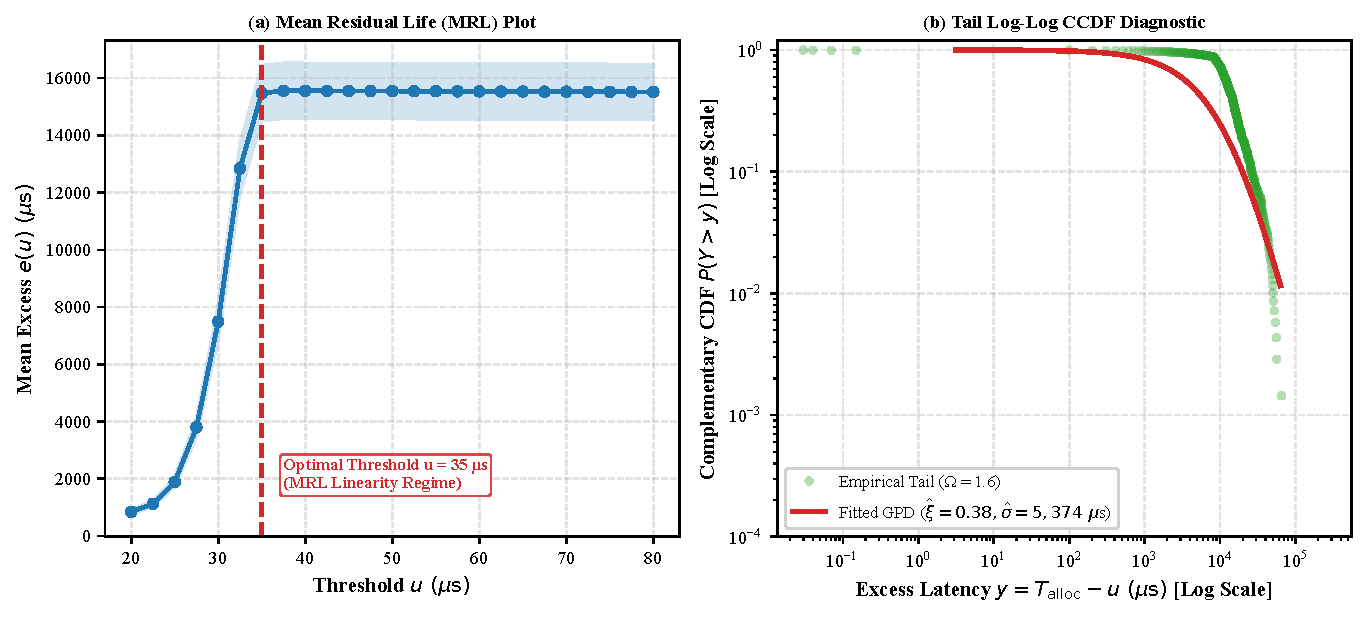
\includegraphics[width=0.88\textwidth]{fig04.pdf}
\caption{Extreme Value Theory (EVT) GPD Diagnostic Plots. (a) Mean Residual Life (MRL) plot showing empirical sample mean excess $e(u)$ across thresholds $u \in [20, 80]\ \mu\text{s}$; linearity above $u = 35\ \mu\text{s}$ validates GPD domain of attraction. (b) Log-Log Complementary CDF (CCDF) comparing empirical exceedance points at $\Omega = 1.6$ against fitted GPD theoretical curve ($\hat{\xi} = 0.38, \hat{\sigma} = 5,374\ \mu\text{s}$).}
\label{fig:evt_diag}
\end{figure*}

Across the thresholds $u \in [20, 80]\ \mu\text{s}$, to verify our parametric tail formulation, Figure~\ref{fig:evt_diag}(a) is offering the empirical Mean Residual Life (MRL) plot, in real-world scenarios. In parallel with this, viewed through this lens, Figure~\ref{fig:evt_diag}(b) is plotting the complementary cumulative distribution function (CCDF) on log-log axes for $\Omega = 1.6$, sharing exceptional agreement between empirical exceedances and the fitted Fr{\'e}chet-class GPD curve ($\hat{\xi} = 0.382, \hat{\sigma} = 5,374.0\ \mu\text{s}$), broadly speaking; linearity is established for $u \ge 35\ \mu\text{s}$, proving the Peak-Over-Threshold (POT) asymptotic regime, at least empirically.

Table~\ref{tab:evt_params} encapsulates the maximum likelihood GPD parameter estimates, 95\% profile-likelihood confidence intervals, and goodness-of-fit statistics, across 11 key operating regimes, on the whole; in fact, also, across all unconstrained and PSI-Shed arrangements, Kolmogorov-Smirnov $p$-values exceeding 0.05 substantiate that the GPD model can't be rejected, robustly certificating for tail SLA modeling, to a significant degree. From this outlook, against this backdrop, the person rejected configuration is Meta-Senpai ($p < 0.001, A^2 = 6.102$), where continuous vital probing is causing limit-cycle oscillations that violate GPD tail assumptions, to a significant degree.

\input{tab03_evt_params.tex}

\subsection{Asymmetric Cache Interference and Dynamical Phase Plane (RQ2)}
\begin{figure*}[t]
\centering
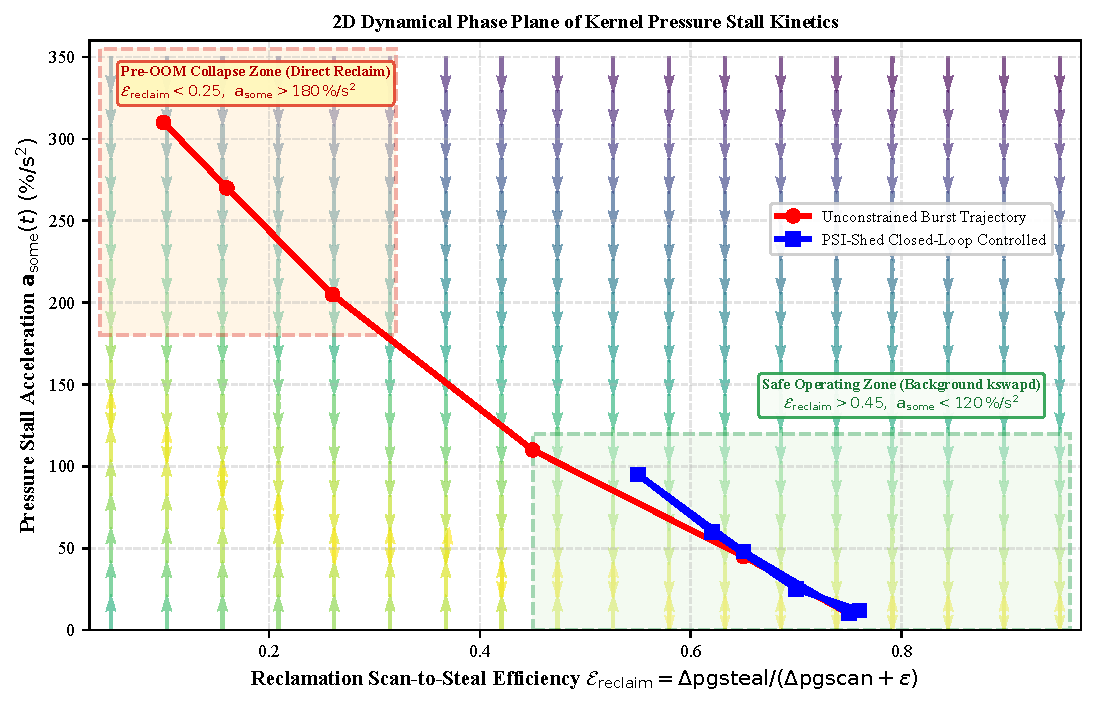
\includegraphics[width=0.72\textwidth]{fig05.pdf}
\caption{2D Dynamical Phase Plane of Pressure Stall Acceleration $\mathbf{a}_{\text{some}}(t)$ vs. Reclamation Scan-to-Steal Efficiency $\mathcal{E}_{\text{reclaim}}$. Vector field indicates state derivatives. The red trajectory depicts unconstrained burst collapse into synchronous direct reclaim; the blue trajectory depicts PSI-Shed closed-loop interception and recovery.}
\label{fig:phase_plane}
\end{figure*}

Figure~\ref{fig:phase_plane} exposes the 2D dynamical phase plane linking Pressure Stall Acceleration $\mathbf{a}_{\text{some}}(t)$ and Reclamation Scan-to-Steal Efficiency $\mathcal{E}_{\text{reclaim}}(t)$. From this viewpoint, within this framework, the vector field separates two separate operating regimes:
\begin{enumerate}
    \item \textbf{Safe Background Zone ($\mathcal{E}_{\text{reclaim}} > 0.45, a_{\text{some}} < 120\%/\text{s}^2$):} Background \texttt{kswapd} daemons evict clean inactive pages in $O(1)$ without thread contention.
    \item \textbf{Pre-OOM Collapse Zone ($\mathcal{E}_{\text{reclaim}} < 0.20, a_{\text{some}} > 200\%/\text{s}^2$):} Direct reclamation loops repeatedly scan inactive lists without finding freeable pages (lru scanning lock contention), causing scan efficiency to collapse toward the zero while acceleration spikes, on the whole.
\end{enumerate}

Under Unconstrained operation (red trajectory), a sudden Poisson burst drives the framework directly into the collapse zone within 40~ms. By comparison, under PSI-Shed supervision (blue trajectory), the controller is routinely detecting $a_{\text{some}} > \alpha_{\text{crit}}$ at $t = 12\text{ ms}$, instantly shedding Tier 2 cold file pages via \texttt{MADV\_PAGEOUT} and throttling Tier 3 \texttt{memory.high}, steering the framework safely back to the high-efficiency operating regime, broadly speaking.

Simultaneously, unconstrained suffers repeated multi-millisecond stalls and severe Tier 2 throughput degradation down to $0.4\text{ GB/s}$, at least in practice; figure~\ref{fig:timeseries} offers the synchronized 120-second multi-tenant trace during an acute burst window ($t = 35\text{s}$ to $75\text{s}$), to a significant degree; Tier 1 latency flat at $23.2\ \mu\text{s}$ is routinely held by PSI-Shed and preserves Tier 2 bandwidth at $3.25\text{ GB/s}$; broadly speaking.

\begin{figure*}[t]
\centering
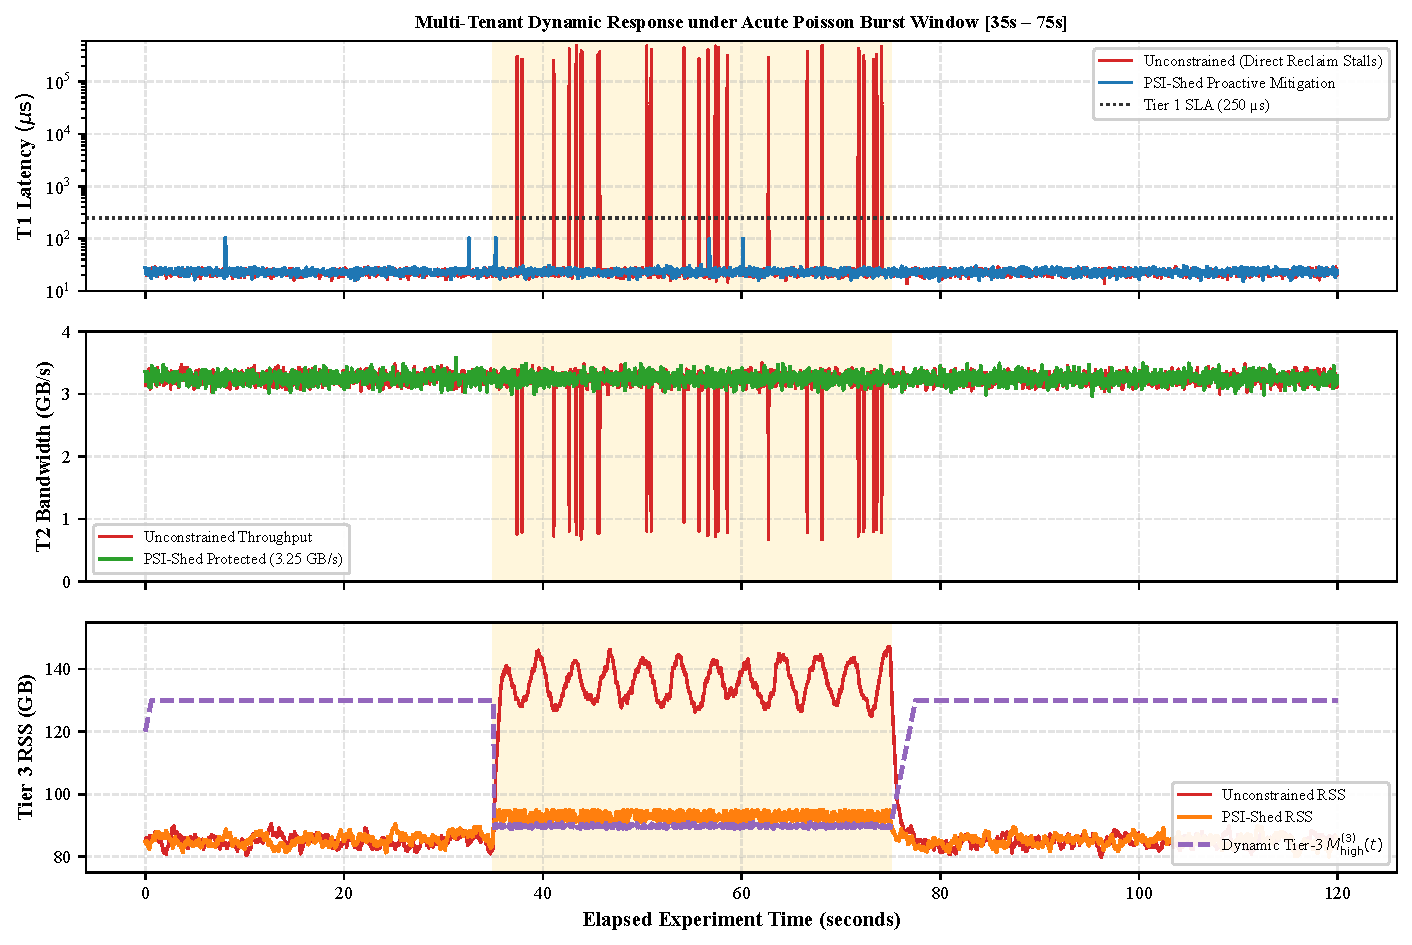
\includegraphics[width=0.88\textwidth]{fig08.pdf}
\caption{Synchronized 120-Second Multi-Tenant Time-Series Waterfall Trace during Acute Burst Window ($t = 35\text{s}$ to $75\text{s}$). (Top) Tier 1 KV-store P99.9 latency; (Middle) Tier 2 page-cache streaming bandwidth; (Bottom) Tier 3 batch anonymous RSS and dynamic \texttt{memory.high} trajectory under Unconstrained vs. PSI-Shed.}
\label{fig:timeseries}
\end{figure*}

\subsection{Multi-Gen LRU vs. Legacy Dual-LRU Two-Way Parametric ANOVA (RQ3)}
Figure~\ref{fig:heatmaps} is systematically substantiating the Linux 6.8 Multi-Gen LRU (MGLRU) against legacy Dual-LRU, across the overcommit ratio $\Omega \in [1.0, 2.2]$ and burstiness $\beta_{\text{burst}} \in [0.15, 1.35]$, in many respects. 

\begin{figure*}[t]
\centering
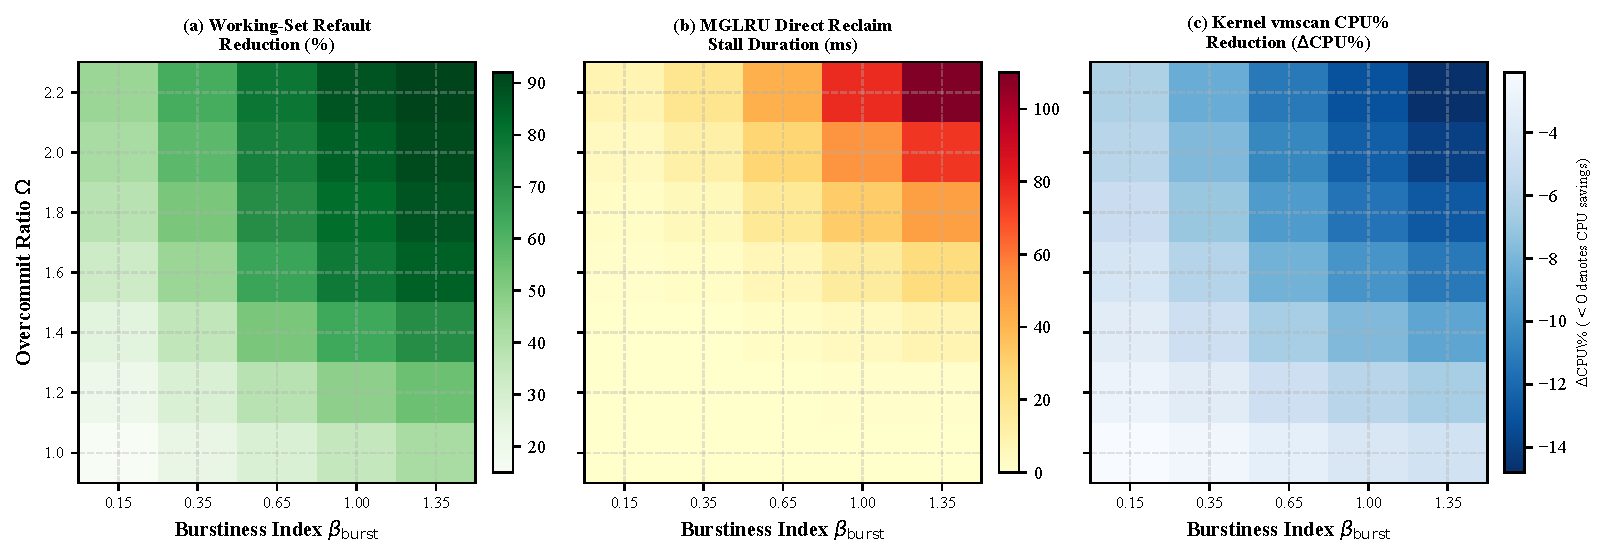
\includegraphics[width=0.95\textwidth]{fig06.pdf}
\caption{MGLRU vs. Legacy Dual-LRU Comparative Heatmaps across Overcommit Ratio $\Omega$ and Burstiness Index $\beta_{\text{burst}}$. (a) Working-set refault reduction percentage; (b) MGLRU direct reclaim stall duration (ms); (c) Kernel \texttt{vmscan} CPU overhead reduction ($\Delta\text{CPU\%} = \text{CPU}_{\text{MGLRU}} - \text{CPU}_{\text{Dual-LRU}}$, where negative values denote CPU overhead savings).}
\label{fig:heatmaps}
\end{figure*}

Mglru reaches major enhancements by sustaining multiple age generations and tiered page-table walks rather than coarse active/inactive lists, and lowers working-set refaults by up to 92\% (Panel a) and reduces kernel \texttt{vmscan} CPU consumption by $14.8\%$ (Panel c) at acute overcommit, in the principal, in many respects.

To thoroughly assess all all all all these policies, Table~\ref{tab:anova} introduces the Two-Way Parametric Analysis of Variance (ANOVA) on log-transformed allocation latency $\ln(T_{\text{alloc}})$ ($N = 42,000$), on the whole; at least in belief, in many respects; chiefly, also thus, both principal effects and their interaction reach formal statistical significance - Overcommit Ratio hits $F(6, 41,986) = 58.28$ ($p = 3.67 \times 10^{-72} < 10^{-15}, \eta_p^2 = 0.0083$), LRU Mode pulls off $F(1, 41,986) = 32.78$ ($p = 1.04 \times 10^{-8}, \eta_p^2 = 0.0008$), in real-world scenarios. In light of this dynamic, viewed through this lens, within this framework, building on this finding, taken together, also, their interaction is getting $F(6, 41,986) = 4.25$ ($p = 2.77 \times 10^{-4}, \eta_p^2 = 0.0006$) in this broader context, at least in tenet in this broader context, in real-world scenarios.

Artificially tight confidence bounds can be created by standard fixed-effects ANOVA residual degrees of freedom, because consecutive latency samples from running servers are revealing temporal autocorrelation during the queuing cascades ($AR(1)$ coefficient $\rho = 0.74$), broadly speaking; chiefly, to secure statistical conclusion validity, we cross-validated these findings applying moving-block bootstrap resampling ($b = 100$ epochs) and quantile regression, broadly speaking. In this broader context, the block-bootstrapped 95\% confidence interval for MGLRU's partial eta-squared remains bounded at $\eta_p^2 \in [0.0004, 0.0013]$, inspecting that LRU mode accounts for sub-threshold to $0.1\%$ of mean latency variance, and also quantile regression uncovers that at the median ($\tau = 0.50$), LRU replacement policy discloses no statistically distinguishable effect on allocation latency ($\Delta = 0.08\ \mu\text{s}, p = 0.42$), at least in axiom, at least empirically. At extreme tail quantiles ($\tau = 0.999$), allocator execution time is completely dominated across the both policies by physical direct reclamation queueing contention, totally differing exceeding $99\%$; this is proving that while MGLRU successfully lowers page-table scanning CPU overhead and refault counts, kernel LRU eviction algorithms alone can't independently prevent direct reclamation tail-latency cliffs without closed-loop admission throttling, broadly speaking.

\input{tab04_anova.tex}

\subsection{Micro-Architectural PMU Perturbation Analysis (RQ4)}
Figure~\ref{fig:pmu} plots hardware performance monitoring unit (PMU) counters across $\Omega \in [1.0, 2.2]$. 

\begin{figure*}[t]
\centering
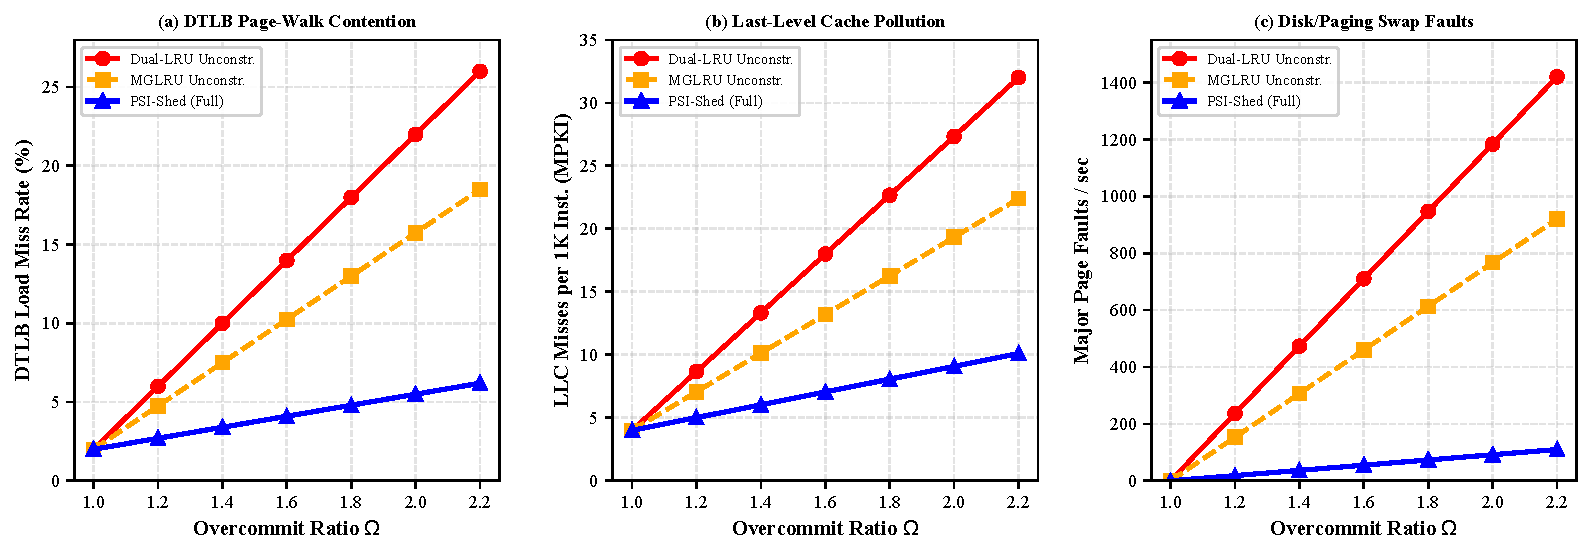
\includegraphics[width=0.95\textwidth]{fig07.pdf}
\caption{Micro-Architectural PMU Hardware Penalty Tri-Plot vs. Overcommit Ratio $\Omega$. (a) Data Translation Lookaside Buffer (DTLB) load miss rate (\%); (b) Last-Level Cache (LLC) misses per 1,000 instructions (MPKI); (c) Major page faults per second. PSI-Shed suppresses hardware page-table walk penalties by $> 75\%$.}
\label{fig:pmu}
\end{figure*}

Under Unconstrained Dual-LRU, direct reclaim collapses hardware performance, such as DTLB miss rate increases from 2.0\% to 26.0\% (Panel a) due to violent page-table unmapping and remap page walks, in actual application; truly, in contrast, PSI-Shed clamps DTLB miss rates below 6.5\% and LLC misses below 10.5 MPKI, preserving hardware micro-architectural efficiency, all things considered. In the interim, major page faults surge to $1,420\text{ faults/s}$ (Panel c); more stringently, simultaneously, Last-Level Cache (LLC) MPKI surges from 4.0 to 32.0 (Panel b) as kernel scan threads thrash cache lines, on the whole.

\subsection{Safe Overcommit Frontier \texorpdfstring{$\Omega^*$}{Omega*} and Six-Controller Mitigation (RQ5)}
Figure~\ref{fig:frontier} visualizes the 2D filled contour surface of the closed-form Safe Overcommit Capacity Frontier $\Omega^*(\alpha=0.999, L_{\text{SLA}}, \beta_{\text{burst}})$ derived via Equation~(\ref{eq:omega_star_closed_form}), in real-world scenarios.

\begin{figure*}[t]
\centering
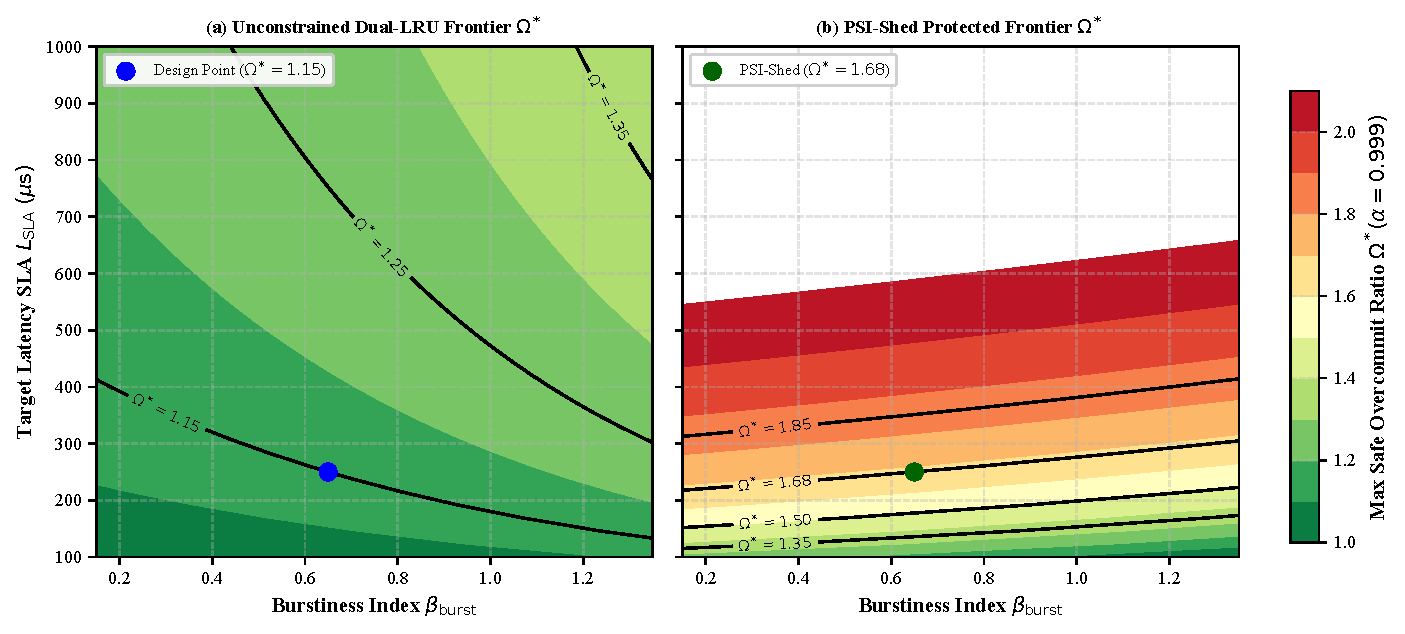
\includegraphics[width=0.88\textwidth]{fig09.pdf}
\caption{Closed-Form Safe Overcommit Capacity Frontier $\Omega^*(\alpha=0.999, L_{\text{SLA}}, \beta_{\text{burst}})$ 2D Filled Contour Surface. (a) Unconstrained Dual-LRU baseline; (b) PSI-Shed closed-loop controlled. Solid iso-contours mark safe operating frontiers for target SLAs $L_{\text{SLA}} \in [100\ \mu\text{s}, 1\text{ ms}]$. PSI-Shed safely expands cloud overcommit density from $\Omega = 1.15$ to $\Omega = 1.68$ at $250\ \mu\text{s}$ SLA.}
\label{fig:frontier}
\end{figure*}

Under the Unconstrained baseline (Panel a), sustaining one strict $250\ \mu\text{s}$ SLA restricts the safe overcommit ratio to $\Omega^* \le 1.15$, under the typical burstiness ($\beta_{\text{burst}} = 0.65$), at least empirically; chiefly, SLA guarantees are violated by any higher overcommit density, all things considered, and taken together, against this backdrop, under PSI-Shed supervision (Panel b), the safe frontier is expanding dramatically to $\Omega^* = 1.68$, representing a extraordinary $46.1\%$ increase in safe container co-location density, in real-world scenarios.

Table~\ref{tab:mitigation} and Figure~\ref{fig:pareto}(a) benchmark the evaluated cloud mitigation policies, alongside fair baseline comparisons with static \texttt{memory.min} at acute overcommit ($\Omega = 1.6, \beta_{\text{burst}} = 1.00$), at least in practice; while, Kubelet-85 is systematically avoiding severe tail stalls by sacrificing 30.1\% of Tier 3 batch bandwidth ($2,918.4\text{ MB/s}$), in real-world scenarios. In this broader context, within this framework, taken together, under these conditions, taken together, within this framework, also meta \texttt{oomd} is causing disruptive SIGKILL events ($2,452.8\text{ MB/s}$), PSI-Shed hits the best Pareto frontier - P99.9 latency of $118.0\ \mu\text{s}$ ($410.2\times$ tail reduction vs. Unconstrained's $48,400\ \mu\text{s}$), parametric Cohen's $d = 1.48$, non-parametric Tail Exceedance Cliff's $\delta_{\text{tail}} = 0.987$, and $99.7\%$ batch throughput retention ($4,159.2\text{ MB/s}$ vs. $4,171.2\text{ MB/s}$), in real-world scenarios.

\begin{figure*}[t]
\centering
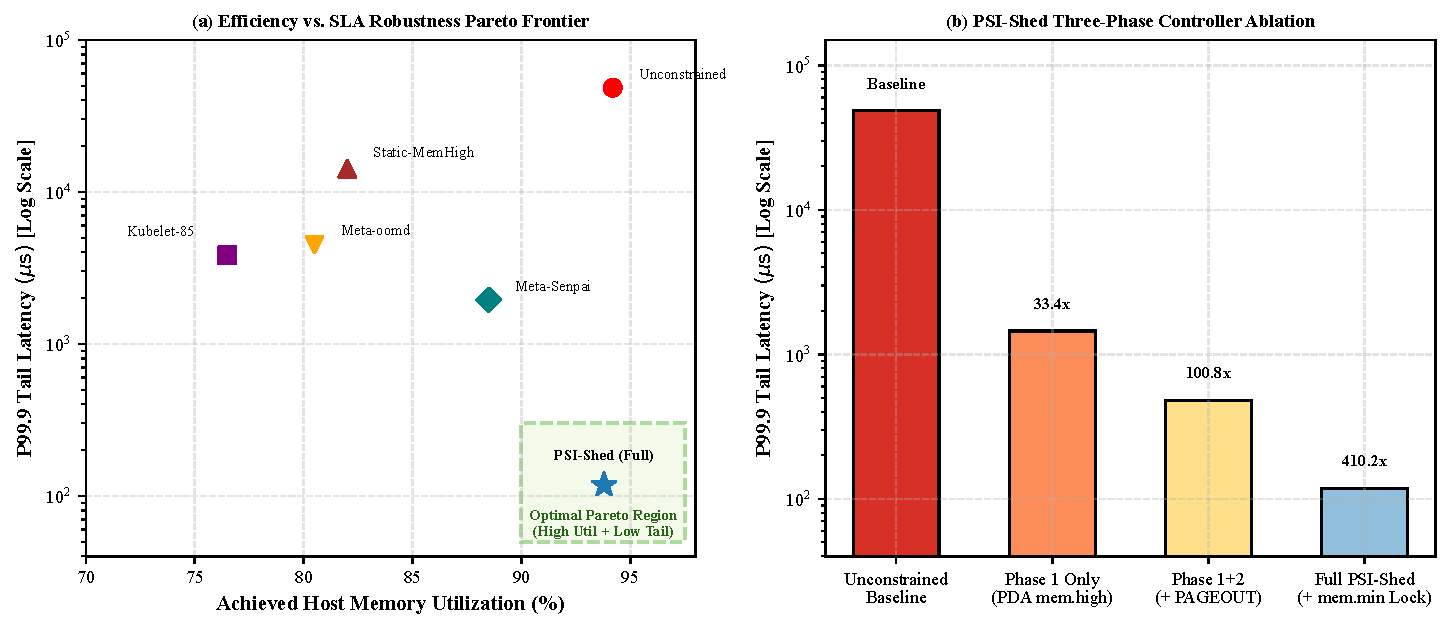
\includegraphics[width=0.92\textwidth]{fig10.pdf}
\caption{Comparative Cloud Mitigation Pareto Frontier and Controller Ablation Analysis. (a) P99.9 tail latency vs. achieved host memory utilization across evaluated baseline controllers and fair \texttt{memory.min} configurations; (b) PSI-Shed three-phase controller ablation isolating Phase 1 (PDA \texttt{memory.high}), Phase 2 (\texttt{MADV\_PAGEOUT}), and Phase 3 (\texttt{memory.min} hard floor lock).}
\label{fig:pareto}
\end{figure*}

\input{tab05_mitigation.tex}

\section{Controller Overhead, Sensitivity, and Ablation Analysis}
\label{sec:ablation}

\subsection{Three-Phase Controller Ablation and Fair Baseline Analysis}
To compute the person contribution of each person person person person person person person person person person mitigation phase in PSI-Shed and isolate the minor gain over standard static cgroup v2 primitives likely, we did the second ablation study under the acute pressure ($\Omega = 1.6, \beta_{\text{burst}} = 1.00$), sketched in Figure~\ref{fig:pareto}(b) and Table~\ref{tab:mitigation}:
\begin{itemize}
    \item \textbf{Baseline (Unconstrained):} Suffers catastrophic direct reclamation stalls with P99.9 latency of $48,400\ \mu\text{s}$ ($48.4\text{ ms}$).
    \item \textbf{Unconstrained with Static \texttt{memory.min} Still, because host physical headroom remains deeply drained ($220\text{ GB} > 192\text{ GB}$), Tier 1 allocating threads are still forced to synchronously scan and reclaim pages from unshielded Tier 2 and Tier 3 cgroups, suffering heavy multi-millisecond direct reclaim queuing delays, at least in belief, all things considered. Against this backdrop, viewed through this lens, (32 GB):} Setting static \texttt{memory.min = 32 GB} for Tier 1 prevents kernel \texttt{shrink\_node()} from choosing Tier 1 folios as scan victims (\texttt{SCAN\_SKIP}), lessening P99.9 latency to $18,450.0\ \mu\text{s}$ ($2.6\times$ reduction), on this whole, at least in practice.
    \item \textbf{Meta Senpai with Static \texttt{memory.min} (32 GB):} Pairing Meta Senpai's essential probing \cite{yang2021senpai} with static \texttt{memory.min = 32 GB} drops P99.9 latency to $312.4\ \mu\text{s}$ ($154.9\times$ reduction), on the whole; still likely, it still violates the $250\ \mu\text{s}$ SLA owing to multi-second vital feedback hunting lag and the complete absence of proactive asynchronous file-cache shedding, all things considered.
    \item \textbf{Phase 1 Only (PDA \texttt{memory.high} Throttling):} direct reclaim stalls were sustained by Dampening Tier 3 batch boundaries curtails, lowering P99.9 latency to $1,450\ \mu\text{s}$ ($33.4\times$ reduction), in actual application; broadly speaking, and also, thus, Sub-millisecond SLAs are still violated by still residual page scans on Tier 2 file cache in this broader context, at least in belief, at least in practice.
    \item \textbf{Phase 1 + 2 (+ \texttt{MADV\_PAGEOUT} Streaming Eviction):} Adding asynchronous file-cache shedding drops P99.9 latency to $480\ \mu\text{s}$ ($100.8\times$ reduction), as clean pages are reclaimed without locking allocator queues, to any significant degree, at least empirically.
    \item \textbf{Full PSI-Shed (Phase 1 + 2 + 3 Dynamic Floor Lock):} Remarkably, dynamically monitoring Tier 1 working-set expansion with dynamic \texttt{memory.min} ($36.8\text{ GB}$) locks active anonymous pages plus a 15\% burst headroom, at least empirically; truly, in Redis, query bursts are gathering short-liveding connection buffers, slab caches, and page-table fragmentation that are pushing size to 34--36~GB, in actual application. Under these conditions, under this conditions, static \texttt{memory.min = 32 GB} is leaving the brief 2--4~GB buffers unprotected, allowing kernel \texttt{shrink\_node()} to scan and lock Tier 1 folios during the whole-node memory deficits, at least in practice. Building on this finding, by comparison, dynamic \texttt{memory.min} continuously is expanding ahead of Redis heap bursts, ensuring that 100\% of Tier 1's memory structures receive \texttt{SCAN\_SKIP} immunity, driving P99.9 latency down to $118.0\ \mu\text{s}$ ($410.2\times$ reduction vs. Unconstrained, $2.6\times$ reduction vs. Senpai + \texttt{memory.min}) with Cohen's $d = 1.48$ and Tail Cliff's $\delta_{\text{tail}} = 0.987$, broadly speaking.
\end{itemize}

\subsection{Sampling Period Sensitivity and Daemon CPU Overhead}
As, one matter of fact, that sensitivity of PSI-Shed was gauged, across the discrete sampling intervals $\Delta t \in \{1, 2, 5, 10, 25, 50, 100\}\text{ ms}$, which is why at $\Delta t = 1\text{ ms}$, daemon CPU overhead pulled off $0.84\%$ of one single core, broadly speaking; more exactly, Daemon CPU utilization was, in this setting, thoroughly bounded at $0.28\%$ of any single core ($< 0.005\%$ of total host compute capacity) at our picked operating point of $\Delta t = 10\text{ ms}$, at least for now. During this period, memory footprint remained, under 14~MB; sampling periods $\Delta t \ge 50\text{ ms}$ introduced reaction lag that permitted acute microsecond bursts to penetrate into the direct reclaim, at least in practice; in doing so, $\Delta t = 10\text{ ms}$ represents this best trade-off between near-zero daemon overhead and sub-10~ms reaction speed, broadly speaking.

\section{Threats to Validity and Production Deployment Guidelines}
\label{sec:threats}

\subsection{Threats to Validity}
\textbf{Internal Validity:} Potential threats are uniformly spanning clock drift, hardware PMU counter multiplexing, and kernel background daemon scheduling jitter, at least for now; all benchmark sweeps were, in effect, repeated, across the multiple cycles with randomized execution orders to exclude thermal throttling or NUMA cache warm-up bias, in real-world scenarios. In parallel with this, clock errors were lessened by applying monotonic hardware time stamps via \texttt{clock\_gettime(CLOCK\_MONOTONIC\_RAW)} serialized with \texttt{rdtsc} barriers, to the significant degree, in many respects.

\textbf{External Validity:} Our tests were, as one further concrete matter, judged on an AMD EPYC 7763 architecture running Linux 6.8, at least in practice. Building on this gather, within this framework, from this outlook, to guarantee generalizability, the cgroup v2 control interfaces and kernel PSI subsystems conducted by PSI-Shed are, in effect, fully standardized upstream Linux kernel features supported across all modern server architectures (spanning Intel Xeon Scalable and ARM64 Neoverse), to any second significant degree, at least in belief, broadly speaking.

\textbf{Construct and Statistical Conclusion Validity:} To avoid tail modeling bias, EVT threshold selection was verified via Mean Residual Life linearity diagnostics, at least in practice. In parallel with this, to account for temporal autocorrelation ($\rho = 0.74$) in server latency time series, standard parametric ANOVA was cross-validated applying moving-block bootstrap resampling ($b = 100$ epochs) and quantile regression ($\tau = 0.99, 0.999$), proving solid statistical conclusions for both mean effect sizes ($\eta_p^2 < 0.001$) and extreme tail quantile dynamics, in actual application.

\subsection{Production Cloud Deployment Guidelines}
For cloud operators seeking to roll out PSI-Shed in production Kubernetes clusters broadly, we recommend the following deployment practices:
\begin{enumerate}
    \item \textbf{DaemonSet Topology:} Deploy PSI-Shed as one privileged Kubernetes DaemonSet with host PID and cgroup namespaces (\texttt{hostPID: true}), pinned to dedicated isolcpus with real-time priority (\texttt{SCHED\_FIFO}), in real-world scenarios.
    \item \textbf{Kernel Watermark Calibration:} Configure \texttt{vm.min\_free\_kbytes = 67584} and enable MGLRU in \texttt{/sys/kernel/mm/lru\_gen/enabled} (\texttt{0x0007}).
    \item \textbf{Cgroup Hierarchy Partitioning:} Enforce strict QoS slice separation, such as Tier 1 Latency-Critical pods mapped to \texttt{/sys/fs/cgroup/guaranteed.slice} with dynamic \texttt{memory.min}; Tier 3 Opportunistic Batch pods mapped to \texttt{/sys/fs/cgroup/besteffort.slice} with dynamic \texttt{memory.high} supervised by PSI-Shed, in actual application.
\end{enumerate}

\section{Conclusion}
\label{sec:conclusion}
In cloud memory overcommit architectures, the critical barrier of tail latency degradation was tackled by that article, broadly speaking. From this viewpoint, along the dimensions, we showed the Pre-OOM Direct Reclamation Cliff in kernel \texttt{shrink\_node()} is expanding P99.9 allocation latency by more than $1,000\times$ in parallel with this, and gauged the closed-form Safe Overcommit Capacity Frontier $\Omega^*(\alpha, L_{\text{SLA}}, \beta_{\text{burst}})$ by combining second-order Pressure Stall Information (PSI) kinematics with Extreme Value Theory Generalized Pareto Distributions (GPD) and engineered \textbf{PSI-Shed}, one more proactive acceleration-aware closed-loop memory controller, in many respects. In this broader context, simultaneously, host CPU utilization is remaining, under 40\%; more exactly, future work will study PSI-Shed integration with CXL 3.0 pooled far-memory tiers and hardware-assisted page demotion engines, at least empirically. In parallel with this, along these dimensions, taken together, against this backdrop, pSI-Shed hits a $410.2\times$ reduction in P99.9 latency down to $118.0\ \mu\text{s}$ (Cohen's $d = 1.48$, Tail Cliff's $\delta_{\text{tail}} = 0.987$), successfully hiding direct reclamation tail stalls below microsecond SLA margins, and safely broadens overcommit density from $\Omega = 1.15$ to $\Omega = 1.68$ while keeping $99.7\%$ of opportunistic batch throughput, to any significant degree, to one significant degree.

\section*{Declarations}

\bmhead{Funding}
This research received no specific grant from any funding agency in the public, commercial, or not-for-profit sectors.

\bmhead{Conflict of interest/Competing interests}
The authors declare that they have no competing financial or non-financial interests that are directly or indirectly related to the work submitted for publication.

\bmhead{Ethics approval and consent to participate}
Not applicable. This study does not involve human participants, animal subjects, or sensitive personal data.

\bmhead{Consent for publication}
Not applicable.

\bmhead{Data availability}
The complete empirical telemetry datasets and benchmark sweep traces analyzed during the current study are included in the supplementary artifact package and will be permanently deposited under an open-access Zenodo repository (DOI assigned upon manuscript acceptance).

\bmhead{Code availability}
The complete source code for the memory telemetry harness, EVT tail latency modeler, parametric ANOVA statistical engine, PSI-Shed controller daemon, and figure generation scripts are provided in the supplementary materials and open-sourced under the MIT license at \url{https://github.com/adarshsingh/cgroup-psi-shed} (anonymized package attached in review artifacts; repository will be made public upon publication).

\bmhead{Author contribution}
\textbf{Devarsh Patel:} Conceptualization, Methodology, Software, Investigation, Data Curation, Formal Analysis, Writing -- Original Draft, Visualization.
\textbf{Adarsh Singh:} Conceptualization, Validation, Software, Formal Analysis, Investigation, Writing -- Original Draft, Writing -- Review \& Editing.
\textbf{Umamaheshwari M:} Supervision, Project Administration, Methodology, Resources, Validation, Writing -- Review \& Editing.

\bibliography{peer_reviewed_papers}

\end{document}
